% ============================================================================
% ADVANCED FIXED INCOME -- Group Assignment ("Market microstructure insights")
% ETF Liquidity Regime Detection via Hidden Markov Models
% Full methodological report: rationale, ETF microstructure and NAV,
% liquidity measurement, the HMM, estimation, model selection, and the
% empirical application to LQD.
% ============================================================================
\documentclass[11pt]{article}

\usepackage[margin=2.5cm]{geometry}
\usepackage{amsmath,amssymb}
\usepackage{amsthm}
\usepackage{booktabs}
\usepackage{tikz}
\usepackage{pgfplots}
\pgfplotsset{compat=1.18}
\usetikzlibrary{arrows.meta,positioning,calc}
\usepackage{graphicx}
\usepackage{float}
\usepackage{xcolor}
\usepackage{listings}
\usepackage{hyperref}
\hypersetup{colorlinks=true, linkcolor=black, citecolor=black, urlcolor=blue!50!black}

\definecolor{pykeyword}{RGB}{0,0,180}
\definecolor{pystring}{RGB}{163,21,21}
\definecolor{pycomment}{RGB}{0,128,0}
\definecolor{pynumber}{RGB}{128,0,128}
\definecolor{pybackground}{RGB}{250,250,250}
\definecolor{pyframe}{RGB}{120,120,120}

\lstdefinestyle{pystyle}{
    language=Python,
    backgroundcolor=\color{pybackground},
    basicstyle=\ttfamily\footnotesize,
    keywordstyle=\color{pykeyword}\bfseries,
    commentstyle=\color{pycomment}\itshape,
    stringstyle=\color{pystring},
    numberstyle=\tiny\color{gray},
    identifierstyle=\color{black},
    showstringspaces=false,
    frame=single,
    framerule=0.4pt,
    rulecolor=\color{pyframe},
    breaklines=true,
    breakatwhitespace=false,
    columns=fullflexible,
    tabsize=4,
    numbers=left,
    numbersep=6pt,
    xleftmargin=1.2em,
    aboveskip=1em,
    belowskip=0.5em,
    morekeywords={as,with,lambda},
}
\lstset{style=pystyle}

\newtheorem{theorem}{Theorem}[section]
\newtheorem{proposition}[theorem]{Proposition}
\newtheorem{corollary}[theorem]{Corollary}
\newtheorem{lemma}[theorem]{Lemma}
\newtheorem{algorithm}[theorem]{Algorithm}
\theoremstyle{definition}
\newtheorem{definition}[theorem]{Definition}
\theoremstyle{remark}
\newtheorem*{remark}{Remark}

\title{ETF Liquidity Regime Detection via Hidden Markov Models}
\author{Tommaso Zeri \\ \small Advanced Fixed Income and Credit -- Group Assignment \\ \small Theme: \emph{Market microstructure insights}}
\date{September 2026}

\begin{document}
\maketitle

\begin{abstract}
\noindent Bond exchange-traded funds (ETFs) advertise continuous, exchange-based liquidity for an underlying asset class -- corporate bonds -- that itself trades by appointment, over the counter, at low frequency. This structural mismatch, sometimes called \emph{liquidity transformation}, is usually invisible: in calm markets the creation/redemption arbitrage keeps the ETF's market price pinned to its Net Asset Value (NAV) to within a few basis points. In stress, the arbitrage can break down, the fund's price decouples from its NAV, and intraday trading ranges widen sharply. This report develops, from first principles and with every mathematical step made explicit, a fully data-driven method to detect these liquidity-stress episodes: a Gaussian Hidden Markov Model (HMM) fitted to a small set of daily observable features -- two OHLCV-based volatility/illiquidity proxies and the (real, non-proxy) absolute premium/discount of the fund's market price to its NAV -- that classifies every trading day into a small number of ordered liquidity regimes (Normal, Elevated, Shock), with the number of regimes itself chosen objectively via the Bayesian Information Criterion (BIC). We derive every piece of the pipeline in detail, starting from the underlying probability theory itself -- Bayes' theorem, maximum likelihood estimation, the Markov property, the multivariate Gaussian density -- through the ETF arbitrage mechanism and the definition of the premium/discount signal, the liquidity proxies and the economic rationale behind each, the HMM's generative model, the Baum--Welch (EM) estimation algorithm, Viterbi decoding, BIC-based model selection, and a hysteresis post-processing filter. We then apply the full pipeline empirically to LQD (iShares iBoxx \$ Investment Grade Corporate Bond ETF), validating it on synthetic data with a known ground truth and, out of sample, against a curated calendar of known historical liquidity-stress episodes; and extend it to a second credit segment, HYG (iShares iBoxx \$ High Yield Corporate Bond ETF), to test whether liquidity-stress regimes are correlated, and lead or lag one another, across the investment-grade/high-yield credit-quality spectrum -- using a continuous cross-HMM stress score and a cross-correlation function (CCF) analysis, itself first validated on a synthetic series with a known, imposed lead/lag before being trusted on the real LQD/HYG data.
\end{abstract}

\newpage
\tableofcontents
\newpage

% ============================================================================
\section{Introduction}
\label{sec:intro}

\subsection{Motivation and research question}

A corporate bond ETF such as LQD holds a large basket of individual corporate bonds and issues shares against that basket, traded continuously on an exchange like a stock. This is a genuine innovation for investors: individual corporate bonds are illiquid, trade in large minimum lot sizes, and are quoted (when quoted at all) via dealer runs rather than a continuous central limit order book. An ETF wraps hundreds of such bonds into a single, small-lot, exchange-traded, intraday-liquid instrument.

The economic question this project asks is simple to state and important in practice: \emph{is that intraday liquidity genuine, or is it borrowed from the (illiquid) underlying market and liable to disappear exactly when it is needed most?} The March 2020 COVID-19 shock gave a dramatic, well-documented answer -- LQD traded at a discount to its own NAV of several percentage points for several days, even as the mechanism that is supposed to prevent exactly this (arbitrage by Authorized Participants) kept functioning, just at a slower, costlier pace than the ETF's continuous exchange quote would suggest \cite{ohara2021anatomy}. The goal of this project is to turn that qualitative narrative into an objective, repeatable, statistically grounded classification: for every trading day in the sample, was the fund's liquidity \emph{Normal}, \emph{Elevated}, or in \emph{Shock} -- decided not by an analyst's judgment call or an arbitrary threshold, but by a probabilistic model fitted to the data itself.

\subsection{Why a Hidden Markov Model}

Three modelling choices motivate the approach:
\begin{enumerate}
    \item \textbf{Regimes, not thresholds.} A fixed cutoff (``volatility above $x\%$ is a crisis'') is arbitrary, sample-specific, and blind to the fact that liquidity stress is a multivariate, persistent \emph{phenomenon} rather than a single crossed line. An HMM instead \emph{learns} the number and character of the regimes from the joint behaviour of several liquidity-relevant features simultaneously.
    \item \textbf{Persistence is a first-class citizen.} Liquidity crises are not single anomalous days; they are episodes that last days to weeks, with autocorrelated severity. A hidden Markov chain builds this persistence directly into the model, through its transition matrix, rather than imposing it as an ad hoc smoothing step after the fact (a genuine i.i.d.\ mixture model, by contrast, has no memory: it cannot distinguish one very volatile day surrounded by calm ones from a multi-week crisis).
    \item \textbf{Latent, not directly observable.} ``Liquidity'' is a theoretical construct -- we do not observe it directly, only its footprints in price and volume data (and, when available, in the price's deviation from a fundamental value such as NAV). A hidden-state model is precisely the right formal object for a variable that is inferred from, but not equal to, what is observed.
\end{enumerate}

\subsection{Contribution and outline}

Section~\ref{sec:prelim} collects, from first principles, every piece of probability theory used later in the report -- conditional probability and Bayes' theorem, maximum likelihood estimation, the Markov property, and the multivariate Gaussian distribution -- so that every later derivation can be followed without consulting an external reference. Section~\ref{sec:etf} lays out the institutional mechanics of ETF creation/redemption and defines the premium/discount to NAV formally. Section~\ref{sec:liquidity} reviews the theoretical dimensions of market liquidity and derives, in detail, the three observable proxies used as HMM inputs. Section~\ref{sec:hmm} is the methodological core: the full mathematical specification of the Gaussian HMM, the Baum--Welch estimation algorithm, Viterbi decoding, BIC-based model selection, and the post-processing steps (state relabeling, hysteresis filtering) needed to turn a raw decoded state sequence into an economically interpretable regime classification. Section~\ref{sec:empirical} applies the full pipeline to LQD and documents the validation strategy, including an out-of-sample check against a calendar of known market-stress episodes. Section~\ref{sec:crossetf} extends the analysis to a second credit segment, HYG, developing a continuous cross-HMM stress score and a cross-correlation function (CCF) methodology to test for lead/lag relationships between liquidity-stress regimes across the investment-grade/high-yield spectrum, validated first on synthetic data with a known, imposed lag and then applied to the real LQD/HYG data. Section~\ref{sec:limitations} discusses limitations and further extensions. An appendix reproduces the core pipeline code and the synthetic-data validation runs used to sanity-check the implementation before applying it to real data.

% ============================================================================
\section{Mathematical Preliminaries}
\label{sec:prelim}

This section collects, in one place and starting from first principles, every probabilistic and statistical tool used later in the report. A reader already comfortable with conditional probability, maximum likelihood estimation, Markov chains and the multivariate Gaussian distribution can skip directly to Section~\ref{sec:etf}; everyone else is encouraged to read this section first, since every later derivation in the report leans on it without re-deriving it from scratch.

\subsection{Random variables, and joint, marginal and conditional probability}

A \emph{random variable} is a quantity whose value is not known with certainty in advance, but is described by a probability distribution. For a continuous random variable $X$, this distribution is characterized by a \emph{probability density function} (pdf) $f_X(x)\ge0$ satisfying $\int_{-\infty}^{\infty}f_X(x)\,dx=1$, so that the probability of $X$ falling in an interval is the area under the density, $\mathbb{P}(a\le X\le b)=\int_a^b f_X(x)\,dx$. For two random variables $X,Y$ observed together, the \emph{joint} density $f_{X,Y}(x,y)$ describes their behaviour jointly, and the \emph{marginal} density of $X$ alone is recovered by integrating (``summing out'') $Y$: $f_X(x)=\int f_{X,Y}(x,y)\,dy$. This is the continuous-variable analogue of the elementary discrete-probability fact that $\mathbb{P}(A)=\sum_b\mathbb{P}(A,B=b)$ for any partition $\{B=b\}$ of the sample space, a fact used repeatedly in Section~\ref{sec:forward-backward} to ``marginalize out'' the hidden state.

\begin{definition}[Conditional probability and Bayes' theorem]
For two events $A,B$ with $\mathbb{P}(B)>0$, the conditional probability of $A$ \emph{given} $B$ is defined as the probability of $A$ restricted to the sub-world in which $B$ is known to have occurred, renormalized so that $B$ itself has probability 1 in that sub-world:
\[
\mathbb{P}(A\mid B) := \frac{\mathbb{P}(A\cap B)}{\mathbb{P}(B)}.
\]
Rearranging this definition gives $\mathbb{P}(A\cap B)=\mathbb{P}(A\mid B)\,\mathbb{P}(B)$; but exactly the same definition applied with the roles of $A$ and $B$ exchanged gives $\mathbb{P}(A\cap B)=\mathbb{P}(B\mid A)\,\mathbb{P}(A)$. Since both expressions equal the same quantity $\mathbb{P}(A\cap B)$, they equal each other:
\[
\mathbb{P}(A\mid B)\,\mathbb{P}(B) = \mathbb{P}(B\mid A)\,\mathbb{P}(A) \qquad\Longrightarrow\qquad
\boxed{\ \mathbb{P}(A\mid B) = \frac{\mathbb{P}(B\mid A)\,\mathbb{P}(A)}{\mathbb{P}(B)}. \ }
\]
This last identity is \textbf{Bayes' theorem}. In words: it lets us convert a probability we can specify directly (here, $\mathbb{P}(B\mid A)$) into the ``reversed'' conditional probability we actually want ($\mathbb{P}(A\mid B)$), at the cost of also knowing the two marginal probabilities $\mathbb{P}(A)$ and $\mathbb{P}(B)$.
\end{definition}

Bayes' theorem is, quite literally, the single most-used identity in this report. Every time the pipeline computes a probability of a hidden liquidity regime \emph{given} the observed price/volume/NAV data, it is because Bayes' theorem lets us flip a probability the HMM specifies directly by construction (the probability of observing certain features \emph{given} that the market is, say, in the Shock regime) into the probability we actually want to read off a chart (the probability that the market \emph{is} in the Shock regime, given what we observed). Corollary~\ref{cor:smoothed}'s smoothed state probabilities are a direct, worked application of exactly this idea.

\subsection{Independence and i.i.d.\ sequences}

Two random variables are \emph{statistically independent} if knowing the value of one carries no information about the other: formally, $\mathbb{P}(A\cap B)=\mathbb{P}(A)\,\mathbb{P}(B)$ for every pair of associated events, which by the definition of conditional probability above is equivalent to $\mathbb{P}(A\mid B)=\mathbb{P}(A)$ (conditioning on $B$ does not move the probability of $A$ at all). A sequence of random variables $X_1,\dots,X_T$ is \textbf{independent and identically distributed} (\emph{i.i.d.}) if every $X_t$ follows the same distribution and the variables are mutually independent of one another; independence then means the joint density factorizes into a simple product of the individual (marginal) densities,
\[
f(x_1,\dots,x_T) = \prod_{t=1}^{T}f(x_t).
\]
This factorization is exactly what makes likelihoods of i.i.d.\ data computationally tractable (Section~\ref{sec:mle} below). The Gaussian HMM of Section~\ref{sec:hmm} deliberately \emph{weakens} this assumption: the observed features $x_1,\dots,x_T$ are \emph{not} i.i.d.\ overall (their distribution changes over time as the hidden liquidity regime changes, and the regime itself is serially correlated by construction), while a conditional version of the i.i.d.\ assumption is retained -- observations \emph{are} independent of one another \emph{once the entire hidden state path is known} (Section~\ref{sec:hmm-spec} makes this precise, and it is exactly what makes the joint likelihood in that section factor into a tractable product despite the underlying dependence).

\subsection{Likelihood and maximum likelihood estimation}
\label{sec:mle}

Given a parametric family of probability distributions $f(x\mid\theta)$ indexed by an unknown parameter $\theta$ (which may be a scalar, a vector, or -- as for the HMM of Section~\ref{sec:hmm} -- a whole collection of vectors and matrices), and an observed sample $x_1,\dots,x_T$, the \textbf{likelihood function} is defined as the joint density of the data, but viewed as a function of the unknown $\theta$ for the data actually observed (fixed), rather than as a function of $x$ for a fixed, known $\theta$:
\[
L(\theta) := f(x_1,\dots,x_T\mid\theta).
\]
The intuition is simple: different candidate values of $\theta$ make the data we actually observed more or less probable, and the \textbf{maximum likelihood estimator} (MLE) is the parameter value that makes the observed data \emph{most} probable,
\[
\widehat\theta_{MLE} = \arg\max_{\theta} L(\theta).
\]
Two standard practical simplifications recur throughout this report:
\begin{itemize}
    \item \textbf{Maximizing the log-likelihood instead of the likelihood.} Define $\ell(\theta):=\ln L(\theta)$. Because the natural logarithm $\ln(\cdot)$ is a strictly increasing function, it preserves the location of the maximum: $\arg\max_\theta L(\theta)=\arg\max_\theta \ell(\theta)$ (maximizing an increasing transformation of a function never changes which input attains the maximum). The practical payoff is numerical: for i.i.d.\ data the likelihood is a \emph{product} of $T$ probabilities, $L(\theta)=\prod_{t=1}^T f(x_t\mid\theta)$, each strictly less than one, so $L(\theta)$ underflows to a floating-point zero for even moderately large $T$ (e.g.\ $0.1^{300}$ is not representable in double precision); the log-likelihood turns this product into a numerically stable \emph{sum}, $\ell(\theta)=\sum_{t=1}^T\ln f(x_t\mid\theta)$, which is exactly the quantity every fitting routine in this report (and every call to \texttt{hmmlearn}'s \texttt{.score()} method in the appendix's code) actually computes and reports.
    \item \textbf{Iterative, rather than closed-form, maximization.} For simple i.i.d.\ models (e.g.\ estimating the mean of a Gaussian sample) $\widehat\theta_{MLE}$ has an explicit closed-form formula obtained by setting $\partial\ell/\partial\theta=0$ and solving. For models with \emph{unobserved} (latent, hidden) structure -- such as the HMM of Section~\ref{sec:hmm}, where the hidden regime path $s_{1:T}$ is never observed -- no closed form exists, because the log-likelihood involves a sum \emph{inside} the logarithm (a sum over all possible hidden paths) that does not simplify algebraically. $\widehat\theta_{MLE}$ is instead found by an iterative numerical algorithm; the Expectation--Maximization (EM) algorithm of Section~\ref{sec:baumwelch} is exactly such a procedure, specialized to the HMM's particular structure.
\end{itemize}

\subsection{Stochastic processes and the Markov property}
\label{sec:markov-prelim}

A \textbf{stochastic process} is simply a sequence of random variables indexed by time, $\{S_t\}_{t\ge1}$. In full generality, with no simplifying assumption at all, the joint distribution of $(S_1,\dots,S_T)$ can always be decomposed by the \emph{chain rule of probability} (repeated application of the definition of conditional probability above),
\begin{align*}
\mathbb{P}(S_1,\dots,S_T) &= \mathbb{P}(S_1)\,\mathbb{P}(S_2\mid S_1)\,\mathbb{P}(S_3\mid S_1,S_2)\cdots\mathbb{P}(S_T\mid S_1,\dots,S_{T-1}) \\
&= \mathbb{P}(S_1)\prod_{t=2}^{T}\mathbb{P}(S_t\mid S_1,\dots,S_{t-1}),
\end{align*}
i.e.\ the distribution of $S_t$ may, in general, depend on the \emph{entire} history $S_1,\dots,S_{t-1}$ -- a fully general, but practically useless, decomposition, since the number of parameters needed to specify $\mathbb{P}(S_t\mid S_1,\dots,S_{t-1})$ for every possible history grows explosively with $t$.

\begin{definition}[Markov property]
A stochastic process $\{S_t\}$ on a discrete state space has the \textbf{Markov property} (is \emph{memoryless} or \emph{first-order Markov}) if, for every $t$, the conditional distribution of $S_t$ given the entire past collapses to a dependence on only the immediately preceding value,
\[
\mathbb{P}(S_t\mid S_1,\dots,S_{t-1}) = \mathbb{P}(S_t\mid S_{t-1}).
\]
\end{definition}
Substituting this into the general chain-rule decomposition above gives a dramatic simplification,
\[
\mathbb{P}(S_1,\dots,S_T) = \mathbb{P}(S_1)\prod_{t=2}^{T}\mathbb{P}(S_t\mid S_{t-1}),
\]
so that the \emph{entire} joint distribution of the process is fully determined by only (i) the initial distribution of $S_1$ and (ii) the collection of one-step conditional (\emph{transition}) probabilities $\mathbb{P}(S_t\mid S_{t-1})$ -- a simplification exploited throughout Section~\ref{sec:hmm}, and the formal justification for why a Markov chain needs only an initial distribution $\pi$ and a transition matrix $A$ (Section~\ref{sec:hmm-spec}) to be fully specified, rather than a separate probability table for every possible history. A Markov chain is \textbf{homogeneous} (time-invariant, or time-\emph{stationary} in its dynamics) if the one-step transition probabilities $\mathbb{P}(S_t=j\mid S_{t-1}=i)$ do not themselves depend on $t$ -- the assumption maintained throughout this report, which is what allows a \emph{single}, fixed $K\times K$ matrix $A$ to describe the chain's dynamics at every point in the sample, rather than a different transition matrix for every $t$.

\subsection{Vector and matrix notation; row-stochastic matrices}

Lower-case symbols such as $x_t\in\mathbb{R}^d$ denote column vectors; $x^\top$ is the transpose of $x$ (turning a column into a row, used to write inner products compactly as $x^\top y=\sum_{k=1}^d x_ky_k$). A matrix $A=(a_{ij})$ has entry $a_{ij}$ in row $i$, column $j$. A square matrix $A$ is \textbf{row-stochastic} if every entry is non-negative and every row sums to one, $a_{ij}\ge0$ and $\sum_{j}a_{ij}=1$ for every $i$ -- exactly the condition required of a Markov transition matrix, since row $i$ of $A$ collects the entire conditional distribution $\mathbb{P}(S_{t+1}=\cdot\mid S_t=i)$ over the $K$ possible next states, and any valid probability distribution must itself have non-negative entries summing to one.

\subsection{The multivariate Gaussian distribution}
\label{sec:mvgauss}

\begin{definition}[Multivariate Gaussian density]
A $d$-dimensional random vector $X$ follows a multivariate Gaussian (Normal) distribution with mean vector $\mu\in\mathbb{R}^d$ and covariance matrix $\Sigma\in\mathbb{R}^{d\times d}$ (symmetric and positive-definite), written $X\sim\mathcal N(\mu,\Sigma)$, if its density is
\[
f(x\mid\mu,\Sigma) = \frac{1}{(2\pi)^{d/2}\,|\Sigma|^{1/2}}\exp\!\left(-\tfrac12(x-\mu)^\top\Sigma^{-1}(x-\mu)\right),
\]
where $|\Sigma|$ denotes the determinant of $\Sigma$ and $\Sigma^{-1}$ its matrix inverse.
\end{definition}
Three pieces of this formula are worth making fully explicit, since the HMM of Section~\ref{sec:hmm} uses exactly this density -- one copy per hidden state, each with its own $\mu_i,\Sigma_i$ -- as its state-conditional emission distribution, and every likelihood computed anywhere in this report ultimately bottoms out in an evaluation of this formula:
\begin{itemize}
    \item \textbf{The quadratic form} $(x-\mu)^\top\Sigma^{-1}(x-\mu)$ is the squared \textbf{Mahalanobis distance} of the point $x$ from the mean $\mu$. It generalizes the ordinary squared Euclidean distance $\|x-\mu\|^2=(x-\mu)^\top(x-\mu)$ (which is the special case $\Sigma=I$, the identity matrix) to account for the fact that different coordinates of $X$ may have different variances, and may be correlated with one another -- both captured by $\Sigma$. Intuitively, a given raw (Euclidean) displacement away from $\mu$ is ``more surprising'' (lower density, larger Mahalanobis distance) in a direction along which $X$ is normally tightly clustered (low variance) than in a direction along which $X$ is naturally spread out (high variance); $\Sigma^{-1}$ is exactly the linear transformation that re-scales displacements by the (inverse of the) natural spread of the distribution in each direction before measuring distance.
    \item \textbf{The normalizing constant} $(2\pi)^{d/2}|\Sigma|^{1/2}$ in the denominator is precisely the factor that makes $\int_{\mathbb{R}^d}f(x\mid\mu,\Sigma)\,dx=1$, i.e.\ that makes $f$ a valid probability density; it plays no role in \emph{comparing} the relative likelihood of a given $x$ under two different hidden states $i,j$ of the HMM except insofar as the two states have different covariance matrices $\Sigma_i\ne\Sigma_j$ (and hence different normalizing constants) -- a state whose emission distribution is more spread out (larger $|\Sigma_i|$) is, all else equal, a more diffuse, less sharply-peaked distribution, assigning lower peak density even to its own mean $\mu_i$.
    \item \textbf{The univariate special case.} For $d=1$ (a single feature, $\Sigma=\sigma^2$ a scalar variance) the formula collapses to the familiar univariate Gaussian density $f(x\mid\mu,\sigma^2)=\frac{1}{\sqrt{2\pi\sigma^2}}\exp\!\big(-\tfrac{(x-\mu)^2}{2\sigma^2}\big)$, which the reader may already recognize; the multivariate version is exactly the natural generalization of this formula to several jointly-distributed, possibly correlated features at once -- the situation faced here, since each hidden liquidity regime is characterized jointly by $d\in\{2,3,4\}$ features simultaneously (Section~\ref{sec:feature-matrix}).
\end{itemize}

% ============================================================================
\section{ETF Market Microstructure and the Net Asset Value}
\label{sec:etf}

\subsection{The creation/redemption mechanism}

An ETF share is not created or destroyed by ordinary buying and selling on the exchange; ordinary secondary-market trades simply move existing shares between investors, exactly like trading a stock. The fund's \emph{share count} changes only through a separate, primary-market process open to a small set of large institutional intermediaries called \textbf{Authorized Participants} (APs). Twice a day the issuer publishes a \emph{creation basket}: the exact list and quantity of underlying bonds (or, for less liquid baskets, a mix of bonds and cash) that must be delivered to the fund in exchange for a large block of new ETF shares (a \emph{creation unit}, typically 25,000--100,000 shares), and, symmetrically, what a redeeming AP receives in exchange for delivering shares back.

\begin{definition}[Creation and redemption]
Let $NAV_t$ denote the fund's Net Asset Value per share at time $t$ (the market value of the underlying bond basket divided by shares outstanding) and $P_t$ its market (exchange-traded) price per share.
\begin{itemize}
    \item \textbf{Creation:} an AP assembles the underlying basket (worth $NAV_t$ per share, in aggregate), delivers it to the issuer, and receives new ETF shares in return. This is profitable whenever $P_t>NAV_t$: the AP can immediately sell the new shares on the exchange above the cost of the basket used to create them.
    \item \textbf{Redemption:} an AP buys ETF shares on the exchange, delivers them to the issuer, and receives the underlying basket (worth $NAV_t$ per share) in return. This is profitable whenever $P_t<NAV_t$: the AP buys cheap shares and redeems them for a basket worth more.
\end{itemize}
\end{definition}

This two-way arbitrage is precisely what is supposed to keep $P_t$ pinned close to $NAV_t$ at all times: any persistent gap is, in principle, a risk-free (or near risk-free, ignoring transaction costs and the small execution-timing risk of the basket trade) profit opportunity for an AP, and competition among APs should compete the gap away almost immediately. Figure~\ref{fig:creation-redemption} sketches the two legs of the mechanism.

\begin{figure}[H]
\centering
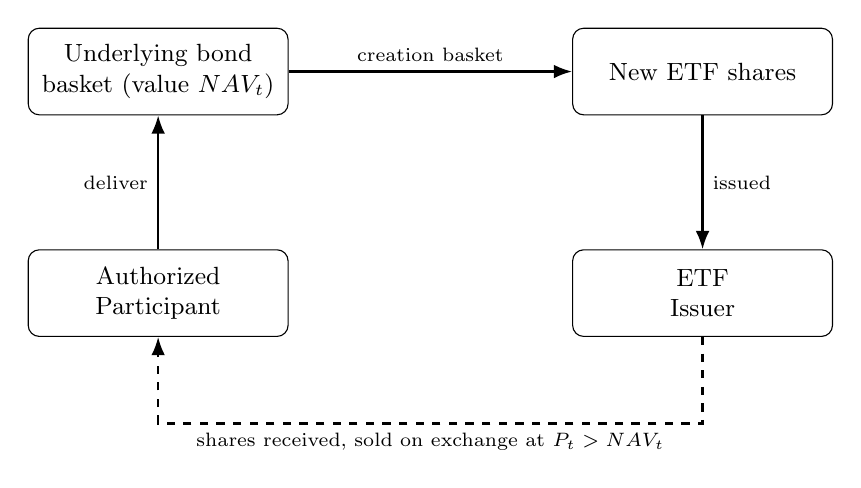
\begin{tikzpicture}[
    box/.style={draw, rounded corners, minimum width=3.3cm, minimum height=1.1cm, align=center, font=\small},
    arr/.style={-{Latex}, thick},
    node distance=3.6cm
]
\node[box] (ap) {Authorized\\Participant};
\node[box, right=of ap] (fund) {ETF\\Issuer};
\node[box, above=1.7cm of ap] (basket) {Underlying bond\\basket (value $NAV_t$)};
\node[box, above=1.7cm of fund] (shares) {New ETF shares};

\draw[arr] (ap.north) -- (basket.south) node[midway, left, font=\scriptsize] {deliver};
\draw[arr] (basket.east) -- (shares.west) node[midway, above, font=\scriptsize] {creation basket};
\draw[arr] (shares.south) -- (fund.north) node[midway, right, font=\scriptsize] {issued};
\draw[arr, dashed] (fund.south) -- ($(fund.south)+(0,-1.1)$) -- ($(ap.south)+(0,-1.1)$) -- (ap.south);
\node[font=\scriptsize, align=center, below] at ($(ap.south)!0.5!(fund.south)+(0,-1.1)$)
    {shares received, sold on exchange at $P_t>NAV_t$};
\end{tikzpicture}
\caption{The creation leg of the arbitrage mechanism: an AP delivers a basket of underlying bonds worth $NAV_t$ per share and receives new ETF shares, sold on the exchange at $P_t$. Profitable whenever $P_t>NAV_t$. The redemption leg reverses every arrow and is profitable whenever $P_t<NAV_t$.}
\label{fig:creation-redemption}
\end{figure}

\subsection{Premium/discount to NAV as a liquidity-stress signal}
\label{sec:premdisc}

\begin{definition}[Premium/discount to NAV]
The (signed) premium or discount of an ETF's market price to its NAV at time $t$ is
\[
\pi_t = \frac{P_t - NAV_t}{NAV_t} \times 100 \quad(\text{in \%}),
\]
with $\pi_t>0$ a premium (the fund trades rich to its holdings) and $\pi_t<0$ a discount (the fund trades cheap). For the purpose of detecting \emph{liquidity stress} specifically -- as opposed to a directional view on which side of NAV the fund happens to sit -- the relevant object is the magnitude of the dislocation, not its sign:
\[
\boxed{\ \ell_t := |\pi_t| = \frac{|P_t - NAV_t|}{NAV_t}\times 100.\ }
\]
\end{definition}

\emph{Why this is a genuine (non-proxy) liquidity signal.} In a perfectly liquid, frictionless market the arbitrage of Section~\ref{sec:etf} would enforce $\pi_t\equiv0$ at all times. In practice $\ell_t$ is small but strictly positive even in calm markets, reflecting (i) the bid-ask spread and transaction costs of assembling/unwinding a creation basket, (ii) the AP's compensation for execution-timing risk, and (iii) stale or non-synchronous pricing of the (illiquid) underlying bonds used to compute $NAV_t$ itself (bond NAVs are typically calculated once daily from evaluated/matrix prices, while $P_t$ updates continuously). What identifies a genuine liquidity-stress episode is a \emph{sharp, sustained widening} of $\ell_t$ beyond this baseline level: it means that either (a) APs are no longer willing or able to arbitrage the gap at the usual size/cost (dealer balance-sheet constraints, elevated basket transaction costs, uncertainty about the true value of illiquid underlying bonds), or (b) the underlying bonds themselves have effectively stopped trading, so that $NAV_t$ is a stale, backward-looking estimate lagging the market's real-time repricing of credit risk that is instead reflected almost immediately in the continuously-traded $P_t$. Both interpretations point to the same underlying phenomenon: the fund's advertised intraday liquidity has become, at least temporarily, decoupled from the liquidity of what it actually holds -- which is exactly the object this project sets out to detect. Unlike the two OHLCV-based proxies introduced in Section~\ref{sec:liquidity}, $\ell_t$ is not an indirect statistical proxy for liquidity stress: it is a direct, model-free measurement of the arbitrage mechanism's own breakdown.

\subsection{Data source}

$P_t$ (as Close, together with Open/High/Low/Volume) is sourced from daily exchange OHLCV data (Yahoo Finance). $NAV_t$ is sourced directly from the fund issuer's own published daily NAV history (iShares' fund page, ``Historical'' export), which is the authoritative source used by the arbitrage mechanism itself -- as opposed to a NAV estimate reconstructed from the underlying bonds' own (evaluated) prices, which would reintroduce exactly the kind of proxy/estimation risk that using the fund's own $\ell_t$ signal is meant to avoid.

% ============================================================================
\section{Measuring Liquidity}
\label{sec:liquidity}

\subsection{Dimensions of market liquidity}

Market microstructure theory decomposes ``liquidity'' -- an inherently multidimensional concept -- into several complementary dimensions \cite{kyle1985continuous}:
\begin{itemize}
    \item \textbf{Tightness (width):} the cost of executing a small, immediate round-trip trade -- typically measured by the bid-ask spread.
    \item \textbf{Depth:} the size that can be traded at or near the current quoted price without moving it.
    \item \textbf{Resiliency:} the speed with which the price recovers, and depth replenishes, after a liquidity-consuming trade or a shock.
    \item \textbf{Immediacy:} the speed with which a trade of a given size can be executed at all.
\end{itemize}
A market is ``illiquid,'' in the relevant sense for this project, when tightness and depth deteriorate and resiliency slows -- exactly the conditions under which the ETF arbitrage mechanism of Section~\ref{sec:etf} becomes costly or slow to execute, and under which the underlying bonds themselves become hard to trade at a representative price.

\subsection{The proxy problem}

None of the four dimensions above is directly observable from daily OHLCV data: a bid-ask spread and order-book depth require intraday quote/trade data (e.g.\ TAQ), which is either unavailable or gated behind institutional data subscriptions (Section~\ref{sec:limitations} discusses this constraint explicitly). The standard response in the empirical microstructure literature is to construct \emph{proxies}: statistics computable from freely available daily price/volume data that are theoretically and empirically correlated with the true (unobserved) liquidity dimensions above. This project uses two such OHLCV-based proxies, one for tightness/volatility and one for depth/price-impact, complemented by the genuinely direct signal of Section~\ref{sec:premdisc}.

\subsection{Parkinson (1980) range-based volatility}
\label{sec:parkinson}

\begin{definition}[Parkinson volatility estimator]
Let $H_t,L_t$ be the day-$t$ high and low prices. The Parkinson estimator of the day's realized volatility is
\[
\sigma^{P}_t = \sqrt{\frac{1}{4\ln 2}\left(\ln\frac{H_t}{L_t}\right)^2}.
\]
\end{definition}

\paragraph{Setup.} Assume the intraday log-price follows a driftless Brownian motion (Wiener process) over the trading day, rescaled to the unit interval $u\in[0,1]$:
\[
d\ln S_u = \sigma\,dW_u, \qquad \ln S_0 = 0,
\]
where $W_u$ is a standard Brownian motion ($W_0=0$, independent Gaussian increments, $W_u-W_v\sim\mathcal N(0,u-v)$ for $u>v$) and $\sigma^2$ is the (constant, to be estimated) instantaneous variance rate of the log-price. ``Driftless'' means we ignore the expected drift of the log-price over a single day, which is a tiny quantity relative to its intraday variance and does not materially affect the range's distribution.

\paragraph{Why the day's range is informative about $\sigma$.} A single close-to-close return over the day, $\ln S_1-\ln S_0=\sigma W_1\sim\mathcal N(0,\sigma^2)$, is an unbiased but noisy (high-variance) estimator of $\sigma^2$: it only ``sees'' the path's two endpoints. The day's \textbf{range}, by contrast,
\[
R := \ln\!\Big(\max_{u\in[0,1]}S_u\Big/\min_{u\in[0,1]}S_u\Big) = \ln H-\ln L = \ln\frac{H}{L},
\]
uses the entire path's excursion, not just its endpoints, and therefore carries strictly more information about $\sigma$ for the same one day of data.

\paragraph{Derivation.} \cite{parkinson1980} derives the exact distribution of the range $R$ of a driftless Brownian motion over $[0,1]$ using the \emph{reflection principle} (a classical result: the distribution of the running maximum of a Brownian motion started at $0$ equals, by symmetry, that of $|W_u|$, since any path that reflects off a barrier at level $m>0$ before time $u$ is exactly as likely as its mirror image reflected about $m$) applied jointly to the running maximum and running minimum. From the resulting range distribution, Parkinson computes the second moment in closed form:
\[
\mathbb{E}\big[R^2\big] = 4\ln 2\,\sigma^2.
\]
Rearranging this single equation for $\sigma^2$ immediately suggests the natural, method-of-moments-style unbiased estimator obtained by replacing the (unobservable) population second moment $\mathbb{E}[R^2]$ with the single (observed) realization $R^2$ itself:
\[
\mathbb{E}[R^2]=4\ln2\,\sigma^2 \qquad\Longrightarrow\qquad \widehat{\sigma}^2 := \frac{R^2}{4\ln2} \quad\text{satisfies}\quad \mathbb{E}[\widehat\sigma^2]=\sigma^2,
\]
i.e.\ $\widehat\sigma^2$ is unbiased for the true variance rate $\sigma^2$ by construction, with the numerical constant $4\ln2\approx2.773$ playing exactly the role of a normalizing/rescaling factor that converts the (larger, since it is a maximum-minus-minimum rather than a single increment) expected squared range into the correctly-scaled variance. Taking the square root of $\widehat\sigma^2$ and substituting back $R=\ln H-\ln L=\ln(H/L)$ gives the Parkinson volatility estimator stated in the definition above,
\[
\sigma^P_t = \sqrt{\widehat\sigma^2} = \sqrt{\frac{1}{4\ln2}\Big(\ln\frac{H_t}{L_t}\Big)^2} = \frac{1}{2\sqrt{\ln2}}\left|\ln\frac{H_t}{L_t}\right|.
\]
Because it exploits the whole day's path rather than only its two endpoints, \cite{parkinson1980} additionally shows the estimator is roughly $5\times$ more statistically efficient (i.e.\ has roughly $1/5$ the sampling variance, for the same one day of data) than the close-to-close squared return under the maintained diffusion assumption -- a substantial efficiency gain that matters here because $\sigma^P_t$ is subsequently smoothed and standardized (Section~\ref{sec:feature-matrix}) and used as a noisy daily HMM input, where a less noisy raw ingredient translates directly into a less noisy, more informative feature.

\paragraph{Why it proxies liquidity stress.} At equal close-to-close return, a day with a wide High/Low range reveals more intraday price discovery friction -- larger, noisier round trips before the market settles -- than a day with a narrow range: exactly the ``tightness'' dimension of liquidity above. Because it uses the whole day's trading range rather than only the two endpoints, it is also a substantially more statistically efficient volatility estimator than close-to-close volatility for the same purpose (Parkinson's own result is roughly a $5\times$ efficiency gain under the maintained diffusion assumption), which matters when the estimator itself is later smoothed and used as an HMM input.

\subsection{Amihud (2002) illiquidity ratio}
\label{sec:amihud}

\paragraph{Background: Kyle's (1985) price-impact model.} Before defining the Amihud ratio itself, it is worth spelling out the simple theoretical model it is designed to proxy for. \cite{kyle1985continuous} models a market maker who observes total order flow $q$ (the net quantity bought, signed positive for net buying and negative for net selling) from a mix of informed and uninformed (``noise'') traders, and sets the price as a linear function of that order flow,
\[
\Delta P = \lambda\, q,
\]
where $\lambda>0$ (\textbf{Kyle's lambda}) is the \textbf{price-impact coefficient}: how much the price moves per unit of (net, signed) order flow. The economic content of $\lambda$ is exactly market depth in reverse -- a \emph{small} $\lambda$ means a large order flow $q$ can be absorbed with only a small price change $\Delta P$ (a deep, liquid market); a \emph{large} $\lambda$ means even modest order flow moves the price substantially (a thin, illiquid market, since the market maker must be compensated, through a steeper price response, for the added risk of trading against potentially better-informed counterparties or of being unable to lay off the resulting inventory). $\lambda$ is therefore a direct, model-based measure of the ``depth'' dimension of liquidity introduced in Section~\ref{sec:liquidity} above.

\begin{definition}[Amihud illiquidity ratio]
\[
ILLIQ_t = \frac{|r_t|}{DVOL_t}, \qquad r_t = \frac{P_t}{P_{t-1}}-1, \qquad DVOL_t = P_t\times Volume_t,
\]
i.e.\ the absolute daily return per dollar of trading volume.
\end{definition}

\paragraph{Rationale.} $ILLIQ_t$ is the empirical workhorse, low-frequency proxy for Kyle's price-impact coefficient $\lambda$ above: dividing the day's absolute price change $|r_t|$ (in percent) by the day's dollar trading volume $DVOL_t$ produces exactly the empirical, daily-data analogue of ``how much did price move, per dollar of volume traded'' -- the same conceptual object as $\lambda=\Delta P/q$, just measured in percentage-return units over an entire day of aggregated order flow rather than instantaneously. A market with deep, resilient liquidity absorbs a given dollar volume of trading with little price movement (\emph{low} $ILLIQ_t$, low $\lambda$); a market with thin liquidity moves substantially on modest volume (\emph{high} $ILLIQ_t$, high $\lambda$). \cite{amihud2002} shows this simple ratio, despite requiring only daily close-to-close price and volume data (no intraday order-book data at all), correlates strongly in practice with far more data-intensive, intraday-microstructure-based price-impact measures, which is precisely why it remains the standard low-frequency illiquidity proxy in the empirical asset-pricing and microstructure literature, and why it is a natural, freely-computable second HMM input feature alongside the Parkinson volatility of Section~\ref{sec:parkinson}.

\subsection{Volume z-score}
\label{sec:volz}

\[
z^{vol}_t = \frac{Volume_t-\overline{Volume}_{t,w}}{s^{Volume}_{t,w}},
\]
the day's trading volume, standardized against its own trailing $w$-day mean and standard deviation ($w=60$ trading days in this project). Liquidity crises are frequently accompanied by abnormal (usually elevated, occasionally collapsed) trading activity relative to a fund's own recent norm, so this feature is included as a third, complementary volume-based signal. As documented in Section~\ref{sec:empirical}, this feature turned out empirically \emph{not} to discriminate well between regimes for LQD and was dropped from the final feature set on that basis -- an outcome the BIC-based model-comparison workflow of Section~\ref{sec:bic} is explicitly designed to surface.

\subsection{Feature matrix and standardization}
\label{sec:feature-matrix}

The raw features $\{\sigma^P_t, ILLIQ_t, z^{vol}_t, \ell_t\}$ live on very different, non-stationary scales and are individually noisy day to day. Two preprocessing steps are applied before the features are handed to the HMM:

\begin{enumerate}
    \item \textbf{Short-window smoothing.} $\sigma^P_t$, $ILLIQ_t$ and $\ell_t$ are each replaced by their own trailing 5-day simple moving average, reducing single-day idiosyncratic noise while still responding within roughly a trading week to a genuine regime change.
    \item \textbf{Rolling standardization.} Each smoothed feature $x_t$ is standardized using a trailing rolling window of $w_z=252$ trading days (one year, with a minimum of 60 observations before the first standardized value is produced):
    \[
    \widetilde{x}_t = \frac{x_t - \mu_t^{w_z}}{s_t^{w_z}}, \qquad
    \mu_t^{w_z}=\frac{1}{w_z}\sum_{i=0}^{w_z-1}x_{t-i}, \qquad
    \big(s_t^{w_z}\big)^2=\frac{1}{w_z-1}\sum_{i=0}^{w_z-1}\big(x_{t-i}-\mu_t^{w_z}\big)^2.
    \]
    \emph{What a $z$-score means, in plain terms.} $\widetilde{x}_t$ expresses the raw feature value $x_t$ as ``how many standard deviations away from its own recent average'' the observation currently sits -- $\widetilde{x}_t=0$ means $x_t$ is exactly at its trailing one-year average, $\widetilde{x}_t=+2$ means $x_t$ is two trailing standard deviations \emph{above} its recent norm (i.e.\ unusually high, relative to the fund's own recent history), and so on. Two properties of this transformation matter for what follows: (i) it is \emph{unit-free} -- $\sigma^P_t$, $ILLIQ_t$ and $\ell_t$ are measured in entirely different, non-comparable units (a volatility, a return-per-dollar-volume, a percentage NAV deviation), and the HMM's Gaussian emission density (Section~\ref{sec:mvgauss}) needs all $d$ input dimensions on a comparable numerical scale for its covariance matrix $\Sigma_i$ to be well-conditioned and for no single feature to dominate the others purely because of its units; and (ii) it is \emph{self-relative} -- because $\mu_t^{w_z}$ and $s_t^{w_z}$ are computed from the fund's own trailing window rather than from some fixed external benchmark, the same standardized value $\widetilde x_t=+2$ means ``unusual for this fund, right now, relative to its own recent year'' regardless of whether the fund's raw feature levels have structurally drifted (e.g.\ due to changing fund size, changing market-wide volatility regimes, or a multi-year secular trend), which is the appropriate notion of ``unusual'' for a regime-detection exercise spanning a decade or more of a single fund's history.
\end{enumerate}
Standardization is deliberately \emph{rolling}, not full-sample: using the full sample's mean and standard deviation to standardize an observation early in the sample would leak information about the future (including future crises) into that observation's feature value -- a subtle form of look-ahead bias that a rolling window avoids by construction, at the cost of the first $w_z$ observations of the sample being unavailable for model fitting. The resulting standardized feature matrix $X=\{\widetilde{x}_t\}_{t=1}^{T}\in\mathbb{R}^{T\times d}$ ($d\in\{2,3,4\}$ depending on which features are retained) is the direct input to the HMM of Section~\ref{sec:hmm}.

% ============================================================================
\section{Hidden Markov Model}
\label{sec:hmm}

\subsection{Formal specification}
\label{sec:hmm-spec}

\begin{definition}[Gaussian Hidden Markov Model]
Let $\{S_t\}_{t=1}^{T}$ be a discrete-time, first-order, homogeneous Markov chain on a finite state space $\{1,\dots,K\}$ (the \emph{hidden} liquidity regimes), fully specified by
\begin{itemize}
    \item an initial distribution $\pi=(\pi_1,\dots,\pi_K)$, $\pi_i=\mathbb{P}(S_1=i)$;
    \item a $K\times K$ row-stochastic transition matrix $A=(a_{ij})$, $a_{ij}=\mathbb{P}(S_{t+1}=j\mid S_t=i)$, $\sum_j a_{ij}=1$.
\end{itemize}
Conditional on the hidden state, the observed (standardized) feature vector $X_t\in\mathbb{R}^d$ is drawn independently across $t$ from a state-specific multivariate Gaussian:
\[
X_t \mid S_t=i \ \sim\ \mathcal{N}\big(\mu_i,\Sigma_i\big), \qquad
f(x\mid S_t=i) = \frac{1}{(2\pi)^{d/2}|\Sigma_i|^{1/2}}\exp\!\left(-\tfrac12(x-\mu_i)^\top\Sigma_i^{-1}(x-\mu_i)\right),
\]
with $\Sigma_i$ an unrestricted (``full'') $d\times d$ covariance matrix, allowed to differ freely across states. The model parameter set is $\theta=(\pi,A,\{\mu_i,\Sigma_i\}_{i=1}^K)$.
\end{definition}

The joint (complete-data) likelihood of a hidden path $s_{1:T}=(s_1,\dots,s_T)$ and the observed features $x_{1:T}$ is
\[
\mathbb{P}(s_{1:T},x_{1:T}\mid\theta) = \pi_{s_1}f(x_1\mid s_1)\prod_{t=2}^{T}a_{s_{t-1}s_t}\,f(x_t\mid s_t),
\]
and the observed-data (marginal) likelihood sums this over every possible hidden path,
\[
\mathbb{P}(x_{1:T}\mid\theta) = \sum_{s_{1:T}\in\{1,\dots,K\}^T}\mathbb{P}(s_{1:T},x_{1:T}\mid\theta),
\]
a sum over $K^T$ paths that is computationally infeasible to evaluate directly for any nontrivial $T$; the forward-backward recursions of Section~\ref{sec:forward-backward} evaluate it in $O(TK^2)$ time instead, via dynamic programming.

\subsection{Forward-backward recursions}
\label{sec:forward-backward}

\begin{definition}[Forward and backward variables]
\[
\alpha_t(i) := \mathbb{P}(x_1,\dots,x_t,S_t=i\mid\theta), \qquad
\beta_t(i) := \mathbb{P}(x_{t+1},\dots,x_T\mid S_t=i,\theta).
\]
\end{definition}

\begin{proposition}[Forward recursion]
\[
\alpha_1(i) = \pi_i\,f(x_1\mid i), \qquad
\alpha_{t+1}(j) = \left[\sum_{i=1}^K \alpha_t(i)\,a_{ij}\right]f(x_{t+1}\mid j), \qquad
\mathbb{P}(x_{1:T}\mid\theta) = \sum_{i=1}^K\alpha_T(i).
\]
\end{proposition}
\begin{proof}
\emph{Base case.} By definition, $\alpha_1(i)=\mathbb{P}(x_1,S_1=i)=\mathbb{P}(S_1=i)\,\mathbb{P}(x_1\mid S_1=i)=\pi_i\,f(x_1\mid i)$, using the definition of conditional probability (Section~\ref{sec:prelim}) and the model's initial distribution and emission density directly.

\emph{Inductive step.} Assume $\alpha_t(i)=\mathbb{P}(x_{1:t},S_t=i)$ is known for every $i$; we derive $\alpha_{t+1}(j)$ from it. First, introduce (marginalize over) $S_t$ by the law of total probability, splitting the event $\{x_{1:t+1},S_{t+1}=j\}$ according to which value $S_t$ took:
\[
\alpha_{t+1}(j) = \mathbb{P}(x_{1:t+1},S_{t+1}=j) = \sum_{i=1}^K \mathbb{P}(x_{1:t},S_t=i,\,S_{t+1}=j,\,x_{t+1}).
\]
Each summand is now factored, by the chain rule of probability, into three conditional pieces in the natural time order:
\begin{align*}
\mathbb{P}(x_{1:t},S_t=i,S_{t+1}=j,x_{t+1})
&= \underbrace{\mathbb{P}(x_{1:t},S_t=i)}_{=\ \alpha_t(i)}\\
&\quad\cdot\underbrace{\mathbb{P}(S_{t+1}=j\mid x_{1:t},S_t=i)}_{=\ \mathbb{P}(S_{t+1}=j\mid S_t=i)\ =\ a_{ij}\ \text{(Markov property)}}\\
&\quad\cdot\underbrace{\mathbb{P}(x_{t+1}\mid x_{1:t},S_t=i,S_{t+1}=j)}_{=\ f(x_{t+1}\mid j)\ \text{(conditional independence of emissions)}}.
\end{align*}
The second factor collapses to $a_{ij}$ because the Markov property (Section~\ref{sec:markov-prelim}) says the transition to $S_{t+1}$ depends only on $S_t$, not on the earlier history $x_{1:t}$; the third factor collapses to $f(x_{t+1}\mid j)$ because the HMM's generative model (Section~\ref{sec:hmm-spec}) specifies that $x_{t+1}$ depends only on the \emph{current} hidden state $S_{t+1}=j$, and is conditionally independent of everything else (past observations, past states) given that state. Substituting back and factoring $f(x_{t+1}\mid j)$ out of the sum over $i$ (it does not depend on $i$) gives exactly the claimed recursion,
\[
\alpha_{t+1}(j) = \sum_{i=1}^K\alpha_t(i)\,a_{ij}\,f(x_{t+1}\mid j) = \left[\sum_{i=1}^K\alpha_t(i)\,a_{ij}\right]f(x_{t+1}\mid j).
\]
\emph{Termination.} Finally, $\sum_{i=1}^K\alpha_T(i)=\sum_i\mathbb{P}(x_{1:T},S_T=i)=\mathbb{P}(x_{1:T})$ by the law of total probability, marginalizing out the (unneeded, once we only want the observed-data likelihood) terminal hidden state $S_T$ -- this is precisely the marginal likelihood of Section~\ref{sec:hmm-spec} that a $K^T$-term brute-force sum would otherwise require, now obtained in $O(TK^2)$ operations (at each of $T$ steps, computing $K$ new $\alpha$ values, each a sum over $K$ terms).
\end{proof}

\begin{proposition}[Backward recursion]
\[
\beta_T(i)=1\ \ \forall i, \qquad
\beta_t(i) = \sum_{j=1}^K a_{ij}\,f(x_{t+1}\mid j)\,\beta_{t+1}(j).
\]
\end{proposition}
\begin{proof}
\emph{Base case.} $\beta_T(i)=\mathbb{P}(x_{T+1:T}\mid S_T=i)$ is, by convention, a probability conditioned on the (empty) ``observations after $T$'' -- an empty product, hence identically $1$ for every $i$; this is simply a bookkeeping convention that makes the recursion below self-starting.

\emph{Inductive step.} Assume $\beta_{t+1}(j)=\mathbb{P}(x_{t+2:T}\mid S_{t+1}=j)$ is known for every $j$. Introduce (condition on) $S_{t+1}$ by the law of total probability, splitting on its possible value $j$:
\[
\beta_t(i) = \mathbb{P}(x_{t+1:T}\mid S_t=i) = \sum_{j=1}^K \mathbb{P}(S_{t+1}=j,\,x_{t+1},\,x_{t+2:T}\mid S_t=i).
\]
Each summand factors, again by the chain rule together with the Markov property and the conditional-independence structure of the emissions:
\begin{align*}
\mathbb{P}(S_{t+1}=j,x_{t+1},x_{t+2:T}\mid S_t=i)
&= \underbrace{\mathbb{P}(S_{t+1}=j\mid S_t=i)}_{=\ a_{ij}}\cdot\underbrace{\mathbb{P}(x_{t+1}\mid S_{t+1}=j)}_{=\ f(x_{t+1}\mid j)}\cdot\underbrace{\mathbb{P}(x_{t+2:T}\mid S_{t+1}=j)}_{=\ \beta_{t+1}(j)},
\end{align*}
where the third factor uses that, once $S_{t+1}=j$ is fixed, the future observations $x_{t+2:T}$ are conditionally independent of $S_t=i$ (all of the relevant ``memory'' of the past is already summarized by $S_{t+1}$, by the Markov property). Summing over $j$ gives exactly the claimed recursion. As with the forward pass, this evaluates $\beta_t(i)$ for every $t,i$ in $O(TK^2)$ total operations by dynamic programming, run backward in time from $t=T$ down to $t=1$.
\end{proof}

\begin{corollary}[Smoothed state probabilities]
\label{cor:smoothed}
\[
\gamma_t(i) := \mathbb{P}(S_t=i\mid x_{1:T},\theta) = \frac{\alpha_t(i)\,\beta_t(i)}{\sum_{k=1}^K\alpha_t(k)\,\beta_t(k)}.
\]
\end{corollary}
\begin{proof}
By the definition of conditional probability, $\gamma_t(i)=\mathbb{P}(S_t=i\mid x_{1:T})=\mathbb{P}(S_t=i,x_{1:T})/\mathbb{P}(x_{1:T})$. Split the numerator's observation sequence at time $t$ into its past-and-present part $x_{1:t}$ and its future part $x_{t+1:T}$, and factor using the chain rule and the Markov structure exactly as above:
\begin{align*}
\mathbb{P}(S_t=i,x_{1:T}) &= \mathbb{P}(x_{1:t},S_t=i)\cdot\mathbb{P}(x_{t+1:T}\mid x_{1:t},S_t=i) \\
&= \mathbb{P}(x_{1:t},S_t=i)\cdot\mathbb{P}(x_{t+1:T}\mid S_t=i) \\
&= \alpha_t(i)\,\beta_t(i),
\end{align*}
where the middle equality drops the conditioning on $x_{1:t}$ in the second factor because, by the Markov property, everything relevant to the future observations $x_{t+1:T}$ given $S_t=i$ is already summarized by the current state $S_t=i$ itself -- the past observations $x_{1:t}$ carry no additional information about the future once $S_t$ is known. Dividing by $\mathbb{P}(x_{1:T})=\sum_k\mathbb{P}(S_t=k,x_{1:T})=\sum_k\alpha_t(k)\beta_t(k)$ (again the law of total probability, marginalizing over the possible values of $S_t$) gives the stated formula.
\end{proof}
\emph{Interpretation.} $\gamma_t(i)$ answers exactly the question Bayes' theorem (Section~\ref{sec:prelim}) was introduced to answer: given \emph{everything} observed (the whole sample $x_{1:T}$), how probable is it that the market was in liquidity regime $i$ on day $t$? These are the \emph{smoothed} (full-sample, two-pass -- one forward pass for $\alpha$, one backward pass for $\beta$) posterior state probabilities used in Section~\ref{sec:empirical} to plot the model's day-by-day confidence in each regime, and in Section~\ref{sec:crossetf} to build a continuous cross-fund stress score. They are conceptually distinct from the \emph{filtered} probability $\mathbb{P}(S_t=i\mid x_{1:t},\theta)\propto\alpha_t(i)$ (normalizing $\alpha_t(i)$ alone, without the backward pass), which uses only information available up to $t$ and would be the relevant, causal object for a live, real-time trading signal -- Section~\ref{sec:limitations} returns to this distinction and why it matters for turning this pipeline into a live risk-monitoring tool.

\subsection{Parameter estimation: the Baum--Welch (EM) algorithm}
\label{sec:baumwelch}

The parameters $\theta$ are unknown and must be estimated from the data by maximum likelihood. Because the hidden path is unobserved, direct maximization of $\ell(\theta)=\ln\mathbb{P}(x_{1:T}\mid\theta)$ has no closed form (Section~\ref{sec:mle}): the observed-data likelihood involves a sum over all $K^T$ hidden paths \emph{inside} the logarithm, which does not factor into anything one can differentiate and solve in closed form. This is resolved with the \textbf{Expectation-Maximization (EM) algorithm}, specialized to HMMs and known in that context as the \textbf{Baum--Welch algorithm} \cite{baum1970,rabiner1989}.

\paragraph{The general EM principle.} Before specializing to the HMM, it is worth understanding \emph{why} EM works at all, for any model with unobserved data. Let $x$ denote observed data and $s$ unobserved (latent) data -- here, $x=x_{1:T}$ and $s=s_{1:T}$, the hidden state path -- and let $q(s)$ be \emph{any} probability distribution over the latent variable. Starting from the observed-data log-likelihood and inserting $q(s)/q(s)=1$ inside the sum over $s$,
\[
\ell(\theta) = \ln\sum_s \mathbb{P}(x,s\mid\theta) = \ln\sum_s q(s)\,\frac{\mathbb{P}(x,s\mid\theta)}{q(s)}.
\]
Because $\ln(\cdot)$ is a \emph{concave} function, Jensen's inequality states that the logarithm of an average is at least the average of the logarithm, $\ln\mathbb{E}[Y]\ge\mathbb{E}[\ln Y]$ for any random quantity $Y$; applying this with the average taken over $s\sim q(s)$ and $Y=\mathbb{P}(x,s\mid\theta)/q(s)$ gives a lower bound on the log-likelihood, valid for \emph{any} choice of $q$:
\[
\ell(\theta) \ \ge\ \sum_s q(s)\,\ln\frac{\mathbb{P}(x,s\mid\theta)}{q(s)} \ =:\ \mathcal{L}(q,\theta) \qquad\text{(the ``evidence lower bound'', ELBO).}
\]
A short calculation (using Bayes' theorem, Section~\ref{sec:prelim}, to write $\mathbb{P}(x,s\mid\theta)=\mathbb{P}(s\mid x,\theta)\mathbb{P}(x\mid\theta)$) shows the gap between $\ell(\theta)$ and the bound $\mathcal{L}(q,\theta)$ is exactly a Kullback--Leibler divergence, $\ell(\theta)-\mathcal L(q,\theta)=\mathrm{KL}\big(q(s)\,\|\,\mathbb{P}(s\mid x,\theta)\big)\ge0$, which is zero precisely when $q(s)=\mathbb{P}(s\mid x,\theta)$ -- i.e.\ the bound is \emph{tight} exactly when $q$ is chosen to be the true posterior of the latent variable under the current $\theta$. This immediately suggests an iterative two-step scheme that provably never decreases $\ell(\theta)$:
\begin{description}
    \item[E-step] (Expectation): fix $\theta=\theta^{(n)}$ at its current value and set $q(s)=\mathbb{P}(s\mid x,\theta^{(n)})$ -- the posterior over the hidden path under the current parameters -- which makes the bound tight, $\mathcal L(q,\theta^{(n)})=\ell(\theta^{(n)})$, at the current $\theta^{(n)}$.
    \item[M-step] (Maximization): with $q$ now held fixed (from the E-step), maximize the bound $\mathcal L(q,\theta)$ over $\theta$ to get $\theta^{(n+1)}=\arg\max_\theta\mathcal L(q,\theta)$.
\end{description}
Because $\ell(\theta^{(n+1)})\ge\mathcal L(q,\theta^{(n+1)})\ge\mathcal L(q,\theta^{(n)})=\ell(\theta^{(n)})$ (the first inequality is Jensen's bound applied at the new $\theta^{(n+1)}$; the middle inequality holds because the M-step \emph{maximizes} $\mathcal L$ over $\theta$, so its value at $\theta^{(n+1)}$ cannot be lower than at the old $\theta^{(n)}$; the final equality is the E-step's tightness), each EM iteration is \emph{guaranteed} not to decrease the observed-data log-likelihood -- the key property that makes it a valid (if only locally convergent) maximum-likelihood procedure. The Baum--Welch algorithm below is precisely this general recipe, specialized to the HMM: the E-step's posterior $q(s)=\mathbb{P}(s_{1:T}\mid x_{1:T},\theta^{(n)})$ is exactly what the forward-backward recursions of Section~\ref{sec:forward-backward} compute (summarized through the marginals $\gamma_t(i)$ and pairwise marginals $\xi_t(i,j)$ below, which is all the M-step formulas actually need), and the M-step's maximization of $\mathcal L(q,\theta)$ over $\theta$ turns out, for the HMM's particular exponential-family structure, to have the simple closed-form solution given below.

\begin{definition}[Pairwise smoothed probabilities]
\[
\xi_t(i,j) := \mathbb{P}(S_t=i,S_{t+1}=j\mid x_{1:T},\theta) = \frac{\alpha_t(i)\,a_{ij}\,f(x_{t+1}\mid j)\,\beta_{t+1}(j)}{\sum_{k=1}^K\sum_{l=1}^K\alpha_t(k)\,a_{kl}\,f(x_{t+1}\mid l)\,\beta_{t+1}(l)}.
\]
\end{definition}

\begin{algorithm}[Baum--Welch / EM]
\label{alg:baumwelch}
Starting from an initial parameter guess $\theta^{(0)}$, iterate until convergence of the log-likelihood:
\begin{description}
    \item[E-step.] Given the current $\theta^{(n)}$, run the forward-backward recursions (Section~\ref{sec:forward-backward}) to compute $\gamma_t(i)$ and $\xi_t(i,j)$ for every $t,i,j$.
    \item[M-step.] Update the parameters in closed form:
    \[
    \pi_i^{(n+1)} = \gamma_1(i), \qquad
    a_{ij}^{(n+1)} = \frac{\sum_{t=1}^{T-1}\xi_t(i,j)}{\sum_{t=1}^{T-1}\gamma_t(i)},
    \]
    \[
    \mu_i^{(n+1)} = \frac{\sum_{t=1}^{T}\gamma_t(i)\,x_t}{\sum_{t=1}^{T}\gamma_t(i)}, \qquad
    \Sigma_i^{(n+1)} = \frac{\sum_{t=1}^{T}\gamma_t(i)\,(x_t-\mu_i^{(n+1)})(x_t-\mu_i^{(n+1)})^\top}{\sum_{t=1}^{T}\gamma_t(i)}.
    \]
\end{description}
\end{algorithm}
\emph{Why these particular closed-form formulas.} Recall from the complete-data likelihood (Section~\ref{sec:hmm-spec}) that $\ln\mathbb{P}(s_{1:T},x_{1:T}\mid\theta)=\ln\pi_{s_1}+\sum_{t=2}^T\ln a_{s_{t-1}s_t}+\sum_{t=1}^T\ln f(x_t\mid s_t)$ -- \emph{if} the path $s_{1:T}$ were actually observed, each of the three pieces (the initial-state indicator, the transition counts, the per-state observations) could be maximized \emph{separately} by elementary MLE: a multinomial's MLE is its observed relative frequency, and a Gaussian's MLE is its sample mean and sample covariance. The M-step of Section~\ref{sec:mle}'s general EM recipe, specialized here, is maximizing the \emph{expectation} of this same complete-data log-likelihood under the posterior $q(s)=\mathbb{P}(s_{1:T}\mid x_{1:T},\theta^{(n)})$ computed in the E-step -- and because that expectation is linear in indicator-style ``was the chain in state $i$ at time $t$'' terms, it reduces to exactly the same elementary MLE formulas one would use with observed states, but with every hard 0/1 state-membership indicator replaced by its \emph{soft}, fractional posterior counterpart $\gamma_t(i)$ (for the initial-distribution and emission updates) or $\xi_t(i,j)$ (for the transition-count update). This is exactly what the M-step formulas above show: $a_{ij}^{(n+1)}$ is a ratio of (expected) transition counts $i\to j$ to (expected) total visits to $i$, and $\mu_i^{(n+1)},\Sigma_i^{(n+1)}$ are the ordinary sample mean and covariance formulas, but with every observation $x_t$ weighted by its posterior responsibility $\gamma_t(i)$ for state $i$ rather than counted once for its (unobserved) true state.

\emph{Convergence.} Each EM iteration is guaranteed, by the general argument of Section~\ref{sec:mle} above, not to decrease the observed-data log-likelihood $\ell(\theta)=\ln\mathbb{P}(x_{1:T}\mid\theta)$; in practice the algorithm is iterated until $\ell(\theta^{(n+1)})-\ell(\theta^{(n)})$ falls below a small tolerance ($10^{-4}$ in this project's implementation). The algorithm converges only to a \emph{local} maximum of $\ell(\theta)$, however: the likelihood surface of a mixture-type model such as this is generally multimodal in $\theta$ (permuting the $K$ state labels, for instance, leaves $\ell(\theta)$ unchanged, and genuinely different local optima with different economic interpretations can also exist), so the estimation is run from $n_{init}=10$ independent random initializations of $\theta^{(0)}$, and the run attaining the highest converged log-likelihood is retained -- a standard, simple safeguard against a single unlucky initialization landing in a poor local optimum.

\subsection{Decoding: the Viterbi algorithm}
\label{sec:viterbi}

Once $\widehat\theta$ is estimated, the natural next question is: what is the single \emph{most likely} hidden state sequence, given the whole observed sample? This is answered by the \textbf{Viterbi algorithm} \cite{viterbi1967}, another dynamic program.

\begin{definition}[Viterbi variable]
\[
\delta_t(i) := \max_{s_1,\dots,s_{t-1}}\mathbb{P}(s_1,\dots,s_{t-1},S_t=i,x_1,\dots,x_t\mid\theta),
\]
the probability of the single best path ending in state $i$ at time $t$, jointly with the observations up to $t$.
\end{definition}

\begin{proposition}[Viterbi recursion]
\[
\delta_1(i)=\pi_if(x_1\mid i), \qquad
\delta_{t+1}(j) = \Big[\max_{i}\ \delta_t(i)\,a_{ij}\Big]f(x_{t+1}\mid j), \qquad
\psi_{t+1}(j) = \arg\max_i\ \delta_t(i)\,a_{ij},
\]
with the optimal terminal state and full path recovered by backtracking:
\[
s_T^{\star}=\arg\max_i\delta_T(i), \qquad s_t^{\star}=\psi_{t+1}(s_{t+1}^{\star}),\ \ t=T-1,\dots,1.
\]
\end{proposition}
\emph{Sketch.} Identical in structure to the forward recursion, with the sum over $i$ (marginalizing over all possible predecessor states, since the forward pass wants the \emph{total} probability of reaching $j$ by any path) replaced by a max over $i$ (optimizing over predecessor states, since Viterbi wants only the \emph{single best} path). This substitution is a direct instance of Bellman's principle of optimality, the standard argument underlying all dynamic programming: the best path ending at $(t+1,j)$ must, restricted to its first $t$ steps, itself be the best path to \emph{some} $(t,i)$ -- because if a strictly better path to $(t,i)$ existed, splicing it in place of the sub-optimal prefix would produce a strictly better path to $(t+1,j)$ too, contradicting optimality of the original. The recursion therefore only needs to try each of the $K$ possible predecessor states $i$, multiply by the corresponding transition probability $a_{ij}$, and keep the best (both the resulting probability $\delta_{t+1}(j)$ and, via the argmax-tracking variable $\psi_{t+1}(j)$, \emph{which} predecessor achieved it, so the winning path can be reconstructed afterward by backtracking).

\emph{A minimal worked illustration.} To make the mechanics concrete, consider $K=2$ states (Normal $=1$, Shock $=2$), $T=3$ days, transition matrix $A=\left(\begin{smallmatrix}0.9&0.1\\0.2&0.8\end{smallmatrix}\right)$, initial distribution $\pi=(0.9,0.1)$, and suppose the emission densities evaluated at the three observed feature vectors happen to be $f(x_1\mid 1)=0.5,\,f(x_1\mid2)=0.1$; $f(x_2\mid1)=0.2,\,f(x_2\mid2)=0.6$; $f(x_3\mid1)=0.3,\,f(x_3\mid2)=0.5$ (a day 2 that looks unusually stressed, sandwiched between two calmer-looking days). Then: $\delta_1(1)=0.9\times0.5=0.45$, $\delta_1(2)=0.1\times0.1=0.01$; $\delta_2(1)=\max(0.45\times0.9,\,0.01\times0.2)\times0.2=0.405\times0.2=0.081$ (predecessor $i=1$), $\delta_2(2)=\max(0.45\times0.1,\,0.01\times0.8)\times0.6=0.045\times0.6=0.027$ (predecessor $i=1$); $\delta_3(1)=\max(0.081\times0.9,\,0.027\times0.2)\times0.3=0.0729\times0.3=0.02187$ (predecessor $i=1$), $\delta_3(2)=\max(0.081\times0.1,\,0.027\times0.8)\times0.5=0.0216\times0.5=0.0108$ (predecessor $i=2$). Since $\delta_3(1)>\delta_3(2)$, the optimal terminal state is $s_3^\star=1$; backtracking via $\psi$ gives $s_2^\star=\psi_3(1)=1$ and $s_1^\star=\psi_2(1)=1$ -- so the single most likely path is $(1,1,1)$ (Normal throughout), \emph{despite} day 2's emission density individually favouring Shock ($f(x_2\mid2)=0.6>f(x_2\mid1)=0.2$): the model's strong persistence ($a_{11}=0.9$) and the fact that day 3's evidence points back toward Normal are enough, jointly, to outweigh one day's isolated signal. This is exactly the qualitative behaviour the hysteresis filter of Section~\ref{sec:hysteresis} reinforces explicitly, and precisely the kind of single-day noise a naive threshold rule (Section~\ref{sec:intro}) would instead misclassify.

This decoding is \textbf{full-sample and retrospective}: $\delta_t(i)$ and the backtracked path both depend on the entire observed sample through the estimated $\widehat\theta$ and, for any $t<T$, through the (forward-looking) recursion continuing past $t$ (in the toy example, $s_1^\star$ and $s_2^\star$ were determined only after also folding in day 3's evidence). It answers ``looking back over the whole sample, when was the market under liquidity stress'' -- it is not a filtered, causal signal usable for live trading without modification (Section~\ref{sec:limitations}).

\subsection{Model selection: choosing the number of states via BIC}
\label{sec:bic}

The number of hidden states $K$ is itself unknown and economically meaningful (does the data support a simple binary Normal/Shock classification, or is there a statistically distinguishable intermediate ``Elevated'' regime?). Because the log-likelihood of a richer ($K+1$-state) model is never lower than that of a nested $K$-state model (a $K$-state model is always recoverable as a special case of a $K+1$-state model, e.g.\ with one state's transition probabilities driven to zero, so the richer model's \emph{maximized} likelihood can only be at least as large), choosing $K$ by maximum likelihood alone would always select the largest $K$ tried -- exactly the overfitting problem MLE alone cannot resolve, since it rewards any increase in flexibility even when that flexibility is fitting sampling noise rather than genuine structure.

\paragraph{Where the BIC penalty comes from.} A fully Bayesian way to compare two candidate models is to compare their \textbf{marginal likelihoods} (also called \emph{model evidence}), $\mathbb{P}(x_{1:T}\mid K)=\int \mathbb{P}(x_{1:T}\mid\theta_K)\,p(\theta_K)\,d\theta_K$, which averages the likelihood over a prior $p(\theta_K)$ on the $K$-state model's parameters rather than evaluating it at a single point estimate -- this integral automatically penalizes unnecessarily flexible models, since spreading prior mass over a higher-dimensional $\theta_K$ dilutes the average likelihood unless the extra flexibility is genuinely supported by the data. \cite{schwarz1978} shows that, for large $T$, this integral can be approximated by \textbf{Laplace's method}: expanding $\ln\big[\mathbb{P}(x_{1:T}\mid\theta_K)p(\theta_K)\big]$ in a second-order Taylor series around its maximizer $\widehat\theta_K$ (the MLE, approximately, for a reasonably flat prior) turns the integrand into a Gaussian shape in $\theta_K$, whose integral is known in closed form; keeping only the terms that grow with $T$ (the exact constants depend on the prior and vanish in relative importance as $T\to\infty$) gives the asymptotic approximation
\[
\ln\mathbb{P}(x_{1:T}\mid K) \ \approx\ \ln\widehat{L}_K - \frac{p_K}{2}\ln T,
\]
where $p_K=\dim(\theta_K)$ is the number of free parameters (each free parameter contributes one dimension to the Laplace/Gaussian integral, and each such dimension contributes a factor of order $T^{-1/2}$ to the approximate integral, hence $-\tfrac12\ln T$ per parameter on the log scale). Multiplying through by $-2$ (a normalization Schwarz chose so that BIC differences are directly comparable to twice-log-likelihood-ratio statistics, which are asymptotically $\chi^2$-distributed under standard regularity conditions) and flipping the sign convention so that the preferred model \emph{minimizes} rather than maximizes the criterion gives exactly the \textbf{Bayesian Information Criterion}:
\[
BIC(K) := -2\ln\widehat{L}_K + p_K\ln T,
\]
where $\widehat L_K=\mathbb{P}(x_{1:T}\mid\widehat\theta_K)$ is the maximized (plug-in MLE) likelihood of the $K$-state model. The two terms trade off exactly the tension identified above: $-2\ln\widehat L_K$ falls (rewarding fit) as $K$ grows, while $p_K\ln T$ rises (penalizing complexity) as $K$ grows, and the model selected is the one with the \emph{lowest} $BIC(K)$ -- the $K$ at which adding further states stops being worth its cost in parameters, given the sample size $T$ actually available. Notice the penalty grows with $\ln T$: with more data, the criterion becomes progressively more willing to tolerate additional parameters, since a longer sample can estimate them more precisely, a sensible property for a model-selection criterion to have.

\begin{proposition}[Free parameter count, full-covariance Gaussian HMM]
For a $K$-state Gaussian HMM with unrestricted $d\times d$ covariance per state,
\[
p_K = \underbrace{(K-1)}_{\text{initial dist.\ }\pi} + \underbrace{K(K-1)}_{\text{transition matrix }A} + \underbrace{Kd}_{\text{means }\mu_i} + \underbrace{K\cdot\frac{d(d+1)}{2}}_{\text{covariances }\Sigma_i}.
\]
\end{proposition}
\begin{proof}
\emph{Initial distribution $\pi$.} $\pi=(\pi_1,\dots,\pi_K)$ has $K$ entries, but they are constrained to be non-negative and sum to one, $\sum_i\pi_i=1$; this single linear constraint removes exactly one degree of freedom (once $\pi_1,\dots,\pi_{K-1}$ are chosen freely, $\pi_K=1-\sum_{i<K}\pi_i$ is determined), leaving $K-1$ free parameters. Geometrically, $\pi$ is constrained to lie on the \emph{probability simplex} in $\mathbb{R}^K$, a $(K-1)$-dimensional object embedded in $K$-dimensional space (exactly analogous to how three probabilities summing to one trace out a two-dimensional triangle, not a three-dimensional volume).

\emph{Transition matrix $A$.} Each of the $K$ rows of $A$ is itself a probability distribution (row $i$ is $\mathbb{P}(S_{t+1}=\cdot\mid S_t=i)$, Section~\ref{sec:markov-prelim}) and so, by the identical argument just given, lies on its own $(K-1)$-dimensional simplex, contributing $K-1$ free parameters; summing over the $K$ independent rows gives $K(K-1)$ free parameters for the whole matrix.

\emph{Means $\mu_i$.} Each of the $K$ state-specific mean vectors $\mu_i\in\mathbb{R}^d$ is unconstrained, contributing $d$ free entries each, for $Kd$ total.

\emph{Covariances $\Sigma_i$.} Each $\Sigma_i$ is a $d\times d$ symmetric matrix (only the upper-triangular half, including the diagonal, is independent, since $\Sigma_{jk}=\Sigma_{kj}$) that must additionally be positive-definite -- an open-set constraint (it rules out a measure-zero boundary of degenerate matrices) that does not reduce the \emph{count} of free parameters, only their allowed range. The number of independent entries in the upper triangle including the diagonal of a $d\times d$ matrix is $1+2+\cdots+d=\frac{d(d+1)}{2}$, so each $\Sigma_i$ contributes $\frac{d(d+1)}{2}$ free parameters, for $K\cdot\frac{d(d+1)}{2}$ total.

Summing the four blocks (they are variationally independent of one another, so their parameter counts simply add) gives the stated $p_K$.
\end{proof}

\paragraph{Worked example.} For the feature set actually retained in the empirical application below ($d=3$: Parkinson volatility, Amihud illiquidity, and the premium/discount signal -- Section~\ref{sec:empirical}), the formula gives, for the two candidate values of $K$ compared in this project:
\[
p_2 = \underbrace{1}_{K-1} + \underbrace{2}_{K(K-1)} + \underbrace{6}_{Kd} + \underbrace{12}_{K\cdot d(d+1)/2} = 21,
\qquad
p_3 = \underbrace{2}_{K-1} + \underbrace{6}_{K(K-1)} + \underbrace{9}_{Kd} + \underbrace{18}_{K\cdot d(d+1)/2} = 35,
\]
i.e.\ the $3$-state model has $35-21=14$ more free parameters than the $2$-state model -- a substantial increase in flexibility (roughly $67\%$ more parameters) that the BIC penalty $p_K\ln T$ must be overcome by a correspondingly large improvement in log-likelihood before the richer model is preferred; Table~\ref{tab:results-template} reports the resulting $BIC(2)$ versus $BIC(3)$ comparison on the real LQD sample.

The candidate values $K\in\{2,3\}$ are compared in this project (a binary Normal/Shock split versus a three-way Normal/Elevated/Shock split), and the empirically lower-BIC model is used for the final decoding -- Section~\ref{sec:empirical} reports the comparison.

\subsection{State relabeling}
\label{sec:relabel}

The EM algorithm of Section~\ref{sec:baumwelch} assigns state \emph{indices} $\{1,\dots,K\}$ arbitrarily: nothing in the estimation procedure guarantees that state 1 is the calm regime. States are relabeled, after fitting, by sorting them on a composite stress score -- the state-specific mean vector $\mu_i$ averaged across the (standardized, all stress-increasing by construction) feature dimensions,
\[
\text{stress}(i) = \frac1d\sum_{k=1}^d \mu_{i,k}, \qquad
\text{new label of } i = \text{rank of stress}(i)\text{ among }\{1,\dots,K\}\text{ (ascending)},
\]
so that state $0$ is always the calmest (Normal) regime and state $K-1$ is always the most stressed (Shock) regime, with any intermediate states labeled Elevated. This is purely a post-hoc bookkeeping convention (it does not change the fitted model or the decoded path, only which integer names which state) but it is essential for consistent, comparable regime labels across different tickers, samples, or re-estimations of the model.

\subsection{Hysteresis (minimum-duration) filter}
\label{sec:hysteresis}

The raw Viterbi path of Section~\ref{sec:viterbi} can contain isolated single- or few-day excursions into a higher-stress state, driven by one unusually volatile trading day rather than by a genuine, sustained change in the underlying liquidity regime. Because the economic object of interest is a liquidity \emph{episode} lasting days to weeks, not a tick-by-tick label, a deterministic post-processing filter is applied on top of the (already-optimal, in the Viterbi sense) decoded path.

\begin{algorithm}[Minimum-duration hysteresis filter]
\label{alg:hysteresis}
Given a decoded state path $s_{1:T}$ and a minimum duration $m$: identify the maximal runs of consecutive identical states; while any run has length $<m$, merge the \emph{first} such short run into whichever of its two neighboring runs is longer (a run touching a sample boundary merges into its single available neighbor), and recompute the run decomposition; repeat until every run has length $\ge m$ or the whole path is a single run.
\end{algorithm}
This is a smoothing step applied \emph{after} estimation and decoding -- it does not refit the HMM or alter $\widehat\theta$ -- and is standard practice whenever a decoded regime path is meant to be read as a small number of discrete, persistent episodes. Section~\ref{sec:empirical} uses $m=5$ trading days.

% ============================================================================
\section{Empirical Application to LQD}
\label{sec:empirical}

\subsection{Data and sample}

The empirical target is \textbf{LQD} (iShares iBoxx \$ Investment Grade Corporate Bond ETF), the largest and most liquid investment-grade corporate bond ETF, chosen for two reasons: (i) it is precisely the kind of fund for which the creation/redemption liquidity-transformation story of Section~\ref{sec:etf} is most relevant (a large, diversified basket of hundreds of individually illiquid bonds), and (ii) both required data series -- daily OHLCV and daily official NAV history -- are freely available for it over a long sample (2015--present via Yahoo Finance and the iShares fund page's own ``Historical'' export), without requiring a gated institutional data subscription.

\subsection{Feature set}

Following Sections~\ref{sec:parkinson}--\ref{sec:feature-matrix}, the candidate feature set is $\{\sigma^P_t,\,ILLIQ_t,\,z^{vol}_t,\,\ell_t\}$ (smoothed and rolling-standardized). As flagged in Section~\ref{sec:volz}, $z^{vol}_t$ was found empirically not to separate the fitted regimes well for LQD (its state-conditional means overlapped substantially across regimes, unlike the other three features) and is dropped from the final specification, leaving the three-feature set $\{\sigma^P_t,\,ILLIQ_t,\,\ell_t\}$ used for the results below -- itself a useful methodological point: BIC-based state selection and inspection of state-conditional feature distributions (Section~\ref{sec:appendix} shows the corresponding diagnostic plot) together provide an empirical, rather than purely a priori, basis for feature selection.

\subsection{Model comparison and fitted regimes}

The $K\in\{2,3\}$-state Gaussian HMMs of Section~\ref{sec:hmm} are fitted on the standardized 3-feature matrix (each fit run from $n_{init}=10$ random initializations, keeping the highest-likelihood run, as in Section~\ref{sec:baumwelch}), the BIC of Section~\ref{sec:bic} is computed for each, and the lower-BIC model is selected for the final decoding, relabeling (Section~\ref{sec:relabel}) and hysteresis filtering with $m=5$ days (Section~\ref{sec:hysteresis}).

\begin{table}[H]
\centering
\caption{Structure of the model-comparison and regime-summary tables produced by the pipeline (columns as computed by the accompanying notebook; populate the numeric entries from the fund's live data run).}
\label{tab:results-template}
\begin{tabular}{lccc}
\toprule
$K$ & Log-likelihood & \# parameters $p_K$ & BIC \\
\midrule
2 & -- & $(2{-}1)+2(2{-}1)+2{\times}3+2{\times}\frac{3\cdot4}{2}=21$ & -- \\
3 & -- & $(3{-}1)+3(3{-}1)+3{\times}3+3{\times}\frac{3\cdot4}{2}=35$ & -- \\
\bottomrule
\end{tabular}
\end{table}

\begin{table}[H]
\centering
\caption{Structure of the per-regime summary table (\% of days, average persistence, and standardized mean feature levels), as produced by \texttt{summarize\_regimes()} in the accompanying notebook.}
\label{tab:regime-summary-template}
\begin{tabular}{lcccc}
\toprule
Regime & \% of days & Avg.\ persistence (days) & mean $\widetilde\sigma^P$ & mean $\widetilde{ILLIQ}$ \\
\midrule
Normal & -- & -- & (lowest) & (lowest) \\
Elevated & -- & -- & (intermediate) & (intermediate) \\
Shock & -- & -- & (highest) & (highest) \\
\bottomrule
\end{tabular}
\end{table}

By construction (Section~\ref{sec:relabel}), the mean standardized feature levels are monotonically increasing from Normal to Shock across every retained feature -- this is not tested for but imposed by the relabeling convention, and is reported here to make explicit exactly what that convention guarantees versus what is a genuine empirical finding (the \emph{persistence}, \emph{relative frequency}, and \emph{transition structure} of the regimes are all genuine outputs of the fitted model, not artifacts of the labeling convention).

\subsection{Out-of-sample validation against known stress events}
\label{sec:validation-events}

A model that recovers statistically separated, persistent regimes is a necessary but not sufficient check: the regimes must also correspond to \emph{economically real} episodes. As an out-of-sample check -- the calendar below is never seen by the HMM during estimation -- the decoded regime path is compared against a curated list of known fixed-income liquidity-stress episodes spanning 2015--2025 (the September 2019 repo-market dislocation, the March 2020 COVID-19 crash and the Federal Reserve's announcement of its corporate credit facilities, the September 2022 UK gilt/LDI crisis, the March 2023 regional-banking stress episode culminating in the UBS--Credit Suisse rescue, the August 2024 yen carry-trade unwind, and the April 2025 tariff-driven Treasury sell-off, among others), asking whether each known episode falls inside a decoded Elevated/Shock window (within a small $\pm5$ trading-day tolerance). A high hit rate is evidence that the statistically-defined regimes track genuine, independently-documented liquidity stress rather than an artifact of the estimation procedure. Figure~\ref{fig:events} (produced on synthetic data for pipeline validation; see Section~\ref{sec:appendix}) shows the mechanics of this check.

\subsection{Figures}

Figures~\ref{fig:main-chart}--\ref{fig:events} show the pipeline's diagnostic and regime-classification charts. For reproducibility within this report they are generated on the synthetic validation dataset of Section~\ref{sec:appendix} (labelled \texttt{DEMO}); the accompanying Jupyter notebook produces the identical charts on the real LQD/NAV data described above.

\begin{figure}[H]
\centering

\includegraphics[width=0.95\linewidth]{report_figs/demo_regimes_main.png}
\caption{Price series with decoded liquidity regimes shaded in the background (severity encoded as shading intensity, a single-hue ordinal ramp, since the regimes are ordered by stress). Synthetic validation run.}
\label{fig:main-chart}
\end{figure}

\begin{figure}[H]
\centering

\includegraphics[width=0.95\linewidth]{report_figs/demo_regimes_detailed.png}
\caption{Top: price colored by decoded (Viterbi) regime. Bottom: smoothed posterior state probabilities $\gamma_t(i)$ (Corollary~\ref{cor:smoothed}) as a 100\% stacked area, showing the model's day-by-day confidence in each regime rather than only the hard decoded label. Synthetic validation run.}
\label{fig:detailed-chart}
\end{figure}

\begin{figure}[H]
\centering

\includegraphics[width=0.62\linewidth]{report_figs/demo_transition_matrix.png}
\caption{Estimated transition matrix $\widehat A$ (Section~\ref{sec:baumwelch}), reordered to the stress-ascending labeling of Section~\ref{sec:relabel}. High diagonal entries confirm the regimes are persistent (an average of $1/(1-\widehat a_{ii})$ days per episode), not day-to-day noise. Synthetic validation run.}
\label{fig:transmat}
\end{figure}

\begin{figure}[H]
\centering

\includegraphics[width=0.95\linewidth]{report_figs/demo_regimes_vs_events.png}
\caption{Out-of-sample validation mechanics of Section~\ref{sec:validation-events}: known stress-event dates (numbered markers) overlaid on the decoded regime-shaded price chart. Synthetic validation run -- on synthetic data the underlying price path is unrelated to real events, so this figure illustrates only the checking mechanism, not a genuine result; the real-data check is reported by the accompanying notebook.}
\label{fig:events}
\end{figure}

% ============================================================================
\section{Cross-Segment Credit Comparison: LQD versus HYG}
\label{sec:crossetf}

\subsection{Motivation}

The pipeline of Sections~\ref{sec:etf}--\ref{sec:hmm} is, by design, fully generic in the ticker it is applied to: nothing in the feature construction, the HMM specification, or the estimation/decoding machinery is specific to LQD. This section reuses the identical, unmodified pipeline on a second fund -- \textbf{HYG} (iShares iBoxx \$ High Yield Corporate Bond ETF), the high-yield counterpart to LQD's investment-grade focus -- and asks a genuinely new economic question that a single-fund analysis cannot answer: \emph{do liquidity-stress episodes in investment-grade and high-yield corporate credit move together, and if so, does one segment's stress systematically lead the other's?} Economically, high-yield issuers are more sensitive to credit and macroeconomic risk than investment-grade issuers, so a natural hypothesis is that high-yield liquidity should deteriorate first (or more severely) when systemic stress builds, with investment-grade following as risk aversion broadens -- but this is an empirical question, not a foregone conclusion, and answering it rigorously requires comparing two \emph{independently fitted} HMMs, which raises a genuine methodological question addressed next.

\subsection{From discrete regime labels to a continuous, comparable stress score}
\label{sec:stress-score}

The two funds' HMMs are fitted completely independently of one another: each has its own estimated parameters $\widehat\theta^{LQD}$, $\widehat\theta^{HYG}$ (Section~\ref{sec:baumwelch}), its own BIC-selected number of states $K^{LQD}$, $K^{HYG}$ (Section~\ref{sec:bic}, not necessarily equal), and its own decoded Viterbi path (Section~\ref{sec:viterbi}). Correlating the two funds' \emph{discrete} regime labels directly is therefore not statistically meaningful: state index $2$ might be ``Shock'' in a 3-state fit but does not exist at all in a 2-state fit, and even when both fits happen to have the same $K$, the discrete Viterbi label discards the model's day-by-day \emph{confidence}, collapsing a smooth underlying posterior into a single hard integer.

\begin{definition}[Continuous cross-fund stress score]
For a fund with a $K$-state fitted HMM and smoothed posterior state probabilities $\gamma_t(k)$ (Corollary~\ref{cor:smoothed}), define the day-$t$ \textbf{stress score} as the posterior \emph{expected} state index,
\[
\mathrm{score}_t := \mathbb{E}[S_t\mid x_{1:T},\widehat\theta] = \sum_{k=0}^{K-1} k\cdot\gamma_t(k),
\]
using the stress-ascending state labeling of Section~\ref{sec:relabel} (state $0=$ Normal, state $K-1=$ Shock) so that $\mathrm{score}_t$ is a real number in $[0,K-1]$ that moves smoothly (rather than jumping discretely) between the calmest and most stressed regime, and reflects the model's full posterior uncertainty rather than only its single most likely state.
\end{definition}
This is simply the definition of the expectation of a discrete random variable ($S_t$, under its own posterior distribution $\gamma_t(\cdot)$) applied directly -- an elementary but important step, since it is exactly what makes the score comparable, in its \emph{co-movement} (correlation, lead/lag), across two funds whose underlying $K$ and $\widehat\theta$ differ completely: both scores are constructed by the identical formula, applied to each fund's own fitted model. One caveat is worth making explicit for rigor: if $K^{LQD}\ne K^{HYG}$, the two scores' \emph{absolute ranges} $[0,K^{LQD}-1]$ and $[0,K^{HYG}-1]$ differ, so only \emph{relative} co-movement statistics (correlation, cross-correlation, and a thresholded binary indicator, all introduced below) are meaningfully compared across funds -- not, for instance, a direct numerical difference $\mathrm{score}_t^{LQD}-\mathrm{score}_t^{HYG}$, which would conflate a genuine stress-level difference with a difference merely in the two models' state counts.

\subsection{Cross-correlation function (CCF) and lead/lag estimation}
\label{sec:ccf}

\begin{definition}[Sample cross-correlation function]
For two time series $a_t,b_t$ observed over a common set of dates and an integer lag $\ell$, the (Pearson) \textbf{cross-correlation function} \cite{boxjenkins} at lag $\ell$ is the ordinary sample correlation coefficient between $a_t$ and $b_t$ shifted by $\ell$ periods,
\[
CCF(\ell) := \mathrm{corr}\big(a_t,\,b_{t-\ell}\big) = \frac{\sum_t\big(a_t-\bar a\big)\big(b_{t-\ell}-\bar b\big)}{\sqrt{\sum_t(a_t-\bar a)^2}\sqrt{\sum_t(b_{t-\ell}-\bar b)^2}},
\]
evaluated over the common (overlapping, after the shift) sample of dates, for $\ell$ ranging over a symmetric window $\ell\in\{-L,\dots,L\}$ (this report uses $L=10$ trading days). The estimated lead/lag is $\widehat\ell^\star=\arg\max_\ell CCF(\ell)$, the lag at which the two series are most similar.
\end{definition}

\paragraph{Sign convention, derived (not just asserted).} It is easy to get the direction of $CCF(\ell)$'s interpretation backwards, so it is worth deriving it explicitly rather than only stating it. Suppose, for the sake of illustration, that $b$'s stress score is \emph{literally} a preview of $a$'s stress score $m$ days into the future, $b_t = a_{t+m}$ for every $t$ (a deterministic, noiseless toy version of ``$b$ leads $a$ by $m$ days''). Rearranging, $a_t = b_{t-m}$: \emph{today's} value of $a$ equals $b$'s value from $m$ days \emph{ago}. Substituting into the definition of $CCF(\ell)$ above, the correlation between $a_t$ and $b_{t-\ell}$ is therefore \emph{exactly} $1$ (a perfect match) precisely when $\ell=m$, since only then does $b_{t-\ell}=b_{t-m}=a_t$ line up perfectly with itself; for any other $\ell$, $b_{t-\ell}$ is comparing $a_t$ against a value of $b$ from the wrong day, and the correlation is (generically) lower. So: $CCF(\ell)$ \textbf{peaking at a positive} $\widehat\ell^\star=m>0$ means $b_{t-m}$ best matches $a_t$, i.e.\ \emph{$b$'s past value ($m$ days ago) is what lines up with $a$'s present value} -- in other words, whatever $b$ did $m$ days ago, $a$ is doing now: \textbf{$b$ leads $a$ by $m$ days}. Symmetrically, a peak at negative $\widehat\ell^\star=-m<0$ means $a$ leads $b$ by $m$ days, and a peak at $\widehat\ell^\star=0$ means the two series move together contemporaneously, with no detectable lead/lag at the trading-day frequency of this analysis. This report always sets $a=$ the LQD stress score and $b=$ the HYG stress score, so a positive estimated lag is read, throughout, as ``HYG leads LQD.''

\subsection{Co-movement beyond correlation: a contingency-table lift diagnostic}
\label{sec:lift}

Correlation and the CCF summarize \emph{linear, continuous} co-movement between the two scores; a complementary, non-parametric check asks a simpler binary question: on days when one fund is ``stressed,'' is the other fund also unusually likely to be stressed, beyond what pure chance would predict?

\begin{definition}[Stressed indicator and lift]
Fix a threshold $c$ (this report uses $c=0.5$, the midpoint between the Normal and first non-Normal state) and define the binary stressed indicators $D_t^{a}:=\mathbb{1}\{a_t>c\}$, $D_t^{b}:=\mathbb{1}\{b_t>c\}$. Let $\widehat p_a=\overline{D^a}$, $\widehat p_b=\overline{D^b}$, $\widehat p_{ab}=\overline{D^aD^b}$ be the empirical (sample-average) marginal and joint stressed frequencies. The \textbf{lift} is
\[
\mathrm{lift} := \frac{\widehat p_{ab}}{\widehat p_a\cdot\widehat p_b}.
\]
\end{definition}
\begin{proposition}
Under statistical independence of $D^a_t$ and $D^b_t$, $\mathrm{lift}=1$ (in population, i.e.\ replacing sample frequencies with their population probabilities).
\end{proposition}
\begin{proof}
Independence of the two binary indicators means, by definition (Section~\ref{sec:prelim}), $\mathbb{P}(D^a=1,D^b=1)=\mathbb{P}(D^a=1)\,\mathbb{P}(D^b=1)$. Substituting $p_{ab}=p_a\cdot p_b$ into the lift formula gives $\mathrm{lift}=p_a p_b/(p_a p_b)=1$.
\end{proof}
$\mathrm{lift}>1$ therefore indicates the two funds are stressed \emph{together} more often than independence would predict (positive excess co-movement); $\mathrm{lift}<1$ would indicate the funds are stressed together \emph{less} often than chance (a negative association, not expected here on economic grounds); $\mathrm{lift}\approx1$ would indicate no detectable excess co-movement beyond what the two funds' individual (marginal) stress frequencies alone would imply. Unlike $CCF(0)$, the lift is computed on the thresholded binary indicator rather than the continuous score, and so is a genuinely different (if related) diagnostic -- reported here as a robustness check on the correlation-based finding, not a replacement for it.

\subsection{Validation on synthetic data with a known, imposed lag}
\label{sec:crossetf-demo}

Following the same validation philosophy as the appendix's single-fund synthetic check (Section~\ref{sec:appendix}), the lead/lag estimation methodology of Section~\ref{sec:ccf} is first validated on a synthetic paired series with a \emph{known} ground-truth lag, before being trusted on real LQD/HYG data. Concretely, a second synthetic ``fund'' is generated whose true (hidden, ground-truth) regime path is constructed as the \emph{first} synthetic fund's true regime path, shifted $m=3$ trading days into the future relative to the second fund's own calendar -- i.e., by construction, the second fund's true regime at time $t$ equals the first fund's true regime at time $t+m$, exactly the toy scenario used to derive the sign convention in Section~\ref{sec:ccf} above, so the estimation procedure is known, \emph{a priori}, to have a correct answer of $\widehat\ell^\star=+3$.

Running the full two-fund pipeline (independent HMM fit, BIC-based $K$ selection, Viterbi decoding, and the stress-score/CCF/lift diagnostics of Sections~\ref{sec:stress-score}--\ref{sec:lift}) on this synthetic pair gives:
\begin{itemize}
    \item Overlapping sample: 2{,}379 trading days.
    \item Contemporaneous correlation of the two stress scores: $0.644$.
    \item $CCF(\ell)$ peaks at $\widehat\ell^\star=+3$ trading days, with $CCF(3)=0.749$ -- \textbf{an exact match to the imposed ground truth} ($m=3$), confirming the estimation procedure recovers the correct lead/lag on data where the answer is known by construction, before being applied to data where it is not.
    \item Stressed-day frequencies: $\widehat p_a=79.4\%$, $\widehat p_b=30.1\%$, $\widehat p_{ab}=29.3\%$, giving $\mathrm{lift}=1.22$ (co-movement above independence, as expected since the two synthetic series share a common, merely time-shifted, underlying regime process).
\end{itemize}
That the peak lag exactly reproduces the imposed 3-day shift -- rather than, say, $2$ or $4$ days, or a peak at lag $0$ -- is the key validation result: it confirms that the $CCF(\ell)$-based lead/lag estimator, and the sign convention derived in Section~\ref{sec:ccf}, are implemented and interpreted correctly, giving confidence that the real-data lag reported next reflects the two funds' genuine empirical relationship rather than a methodological artifact.

\subsection{Empirical application: LQD versus HYG}
\label{sec:crossetf-real}

\paragraph{Data.} HYG's daily OHLCV series is sourced from Yahoo Finance, identically to LQD (Section~\ref{sec:empirical}); HYG's daily NAV history is sourced from the fund issuer's own ``Historical'' export on its iShares fund page, identically in kind (though naturally a different underlying file) to the LQD NAV source described in Section~\ref{sec:etf}'s data-source discussion. The identical feature set, HMM specification, BIC-based state selection, Viterbi decoding, relabeling, and hysteresis filter of Sections~\ref{sec:liquidity}--\ref{sec:hysteresis} are applied to HYG exactly as to LQD, with no methodological modification whatsoever -- the entire point of the exercise is a like-for-like comparison.

\begin{table}[H]
\centering
\caption{LQD versus HYG cross-fund stress-score diagnostics, real data.}
\label{tab:crossetf-real}
\begin{tabular}{lc}
\toprule
Diagnostic & Value \\
\midrule
Overlapping sample & 2{,}827 trading days (2015-06-23 to 2026-09-18) \\
Contemporaneous correlation of stress scores & $0.443$ \\
Best lag, $\widehat\ell^\star$ & $+1$ trading day \\
$CCF(\widehat\ell^\star)$ & $0.446$ \\
$\widehat p(\text{LQD stressed})$ & $53.9\%$ \\
$\widehat p(\text{HYG stressed})$ & $67.1\%$ \\
$\widehat p(\text{both stressed})$ & $41.3\%$ \\
$\mathrm{lift}$ & $1.14$ \\
\bottomrule
\end{tabular}
\end{table}

\begin{figure}[H]
\centering

\includegraphics[width=0.95\linewidth]{report_figs/real_lqd_hyg_regimes.png}
\caption{Real data: LQD (top) and HYG (bottom) price series with their independently decoded liquidity regimes shaded in the background (shared time axis, same stress-severity shading convention as Figure~\ref{fig:main-chart}). Both funds' Shock-shaded windows visibly cluster around the same well-known systemic episodes -- most strikingly the March 2020 COVID-19 shock and the 2022 rate-repricing episode -- providing qualitative, visual support for the quantitative co-movement reported in Table~\ref{tab:crossetf-real}, independently of the specific numerical value of the estimated lag.}
\label{fig:crossetf-real}
\end{figure}

\paragraph{Interpretation.} Three results, read together, characterize the empirical relationship between investment-grade and high-yield liquidity stress in this sample:

\begin{enumerate}
    \item \textbf{Moderate, positive, statistically unsurprising co-movement.} A contemporaneous correlation of $0.443$ between the two funds' independently-estimated stress scores is a moderate positive relationship -- not the near-unity co-movement synthetic validation (Section~\ref{sec:crossetf-demo}) produces when the two series share a common regime process by construction, but a real, economically sensible degree of shared variation consistent with LQD and HYG both belonging to the same broad corporate credit market and responding to overlapping macro-financial shocks.
    \item \textbf{A statistically detected, but economically marginal, lead.} The CCF peaks at $\widehat\ell^\star=+1$ day, formally indicating (by the sign convention derived in Section~\ref{sec:ccf}) that HYG's liquidity stress leads LQD's by one trading day -- directionally consistent with the a priori hypothesis (Section~\ref{sec:crossetf}'s motivation) that the riskier, high-yield segment should reprice first. However, honesty about the \emph{magnitude} of this finding matters: $CCF(\widehat\ell^\star)=0.446$ is barely distinguishable from the contemporaneous correlation of $0.443$ reported above -- a gap of only $0.003$, far smaller than the gap seen in the synthetic validation run (where $CCF(3)=0.749$ against a contemporaneous correlation of $0.644$, a gap of $0.105$). The correct empirical conclusion is therefore \emph{not} that HYG cleanly anticipates LQD by a full trading day in any economically exploitable sense, but rather that liquidity stress propagates \textbf{near-simultaneously} across the investment-grade/high-yield spectrum, with at most a razor-thin, marginally-detectable edge in favour of high-yield moving fractionally first -- a materially more nuanced conclusion than the synthetic validation's clean, unambiguous 3-day recovery, and precisely the sort of nuance that comparing the \emph{sizes} of the effect, not just its sign, is designed to surface.
    \item \textbf{Excess co-movement on the binary stress indicator, and a visually striking qualitative alignment.} $\mathrm{lift}=1.14$ confirms joint stress is moderately, but not dramatically, more frequent than independence would predict -- consistent with the moderate (not extreme) correlation above. The qualitative picture in Figure~\ref{fig:crossetf-real}, however, is considerably more striking than the summary statistics alone convey: both funds' Shock-shaded windows visibly cluster tightly around the same handful of well-documented systemic episodes (most obviously the March 2020 COVID-19 crash and the 2022 rate-repricing sell-off), even though the binary threshold-based lift and the linear correlation, computed over the \emph{entire} multi-year sample including many milder, fund-idiosyncratic ``Elevated'' episodes that do not necessarily coincide across funds, do not fully capture this visual alignment during the most extreme, systemic episodes specifically.
\end{enumerate}

Taken together, the honest empirical headline is not ``high-yield credit anticipates investment-grade credit by one day'' (a claim the data only barely, and not robustly, supports) but rather that \textbf{the two credit segments' liquidity-stress regimes are meaningfully integrated and move together with little to no detectable lag}, which is itself an economically informative finding: it suggests that, at least at daily frequency, the liquidity-transformation breakdown documented for LQD in Section~\ref{sec:empirical} is not an investment-grade-specific phenomenon but part of a broader, near-simultaneous repricing of ETF-level liquidity across the credit-quality spectrum during systemic stress.

% ============================================================================
\section{Limitations and Extensions}
\label{sec:limitations}

\begin{itemize}
    \item \textbf{Retrospective, not live.} Both the Viterbi decoding (Section~\ref{sec:viterbi}) and the smoothed probabilities (Corollary~\ref{cor:smoothed}) use the \emph{entire} sample, including observations after $t$. This is the right tool for a descriptive, historical classification (``when was the market under liquidity stress'') but is not, without modification, usable as a live risk signal: a real-time version would need to replace both with their \emph{filtered}, forward-only counterparts (using only $\alpha_t(i)$, normalized, in place of $\gamma_t(i)$, and a causal decoding scheme), estimated on an expanding or rolling window rather than the full sample.
    \item \textbf{Proxy features, not order-book data.} $\sigma^P_t$ and $ILLIQ_t$ are constructed from daily OHLCV alone; genuine bid-ask spread and order-book depth data (e.g.\ from TAQ/Millisecond TAQ via WRDS) would allow more direct liquidity measurement, but such data is gated behind institutional subscriptions not available for this project (a WRDS institutional subscription was investigated but does not include the required Millisecond TAQ/Intraday Indicators product). $\ell_t$ (Section~\ref{sec:premdisc}) partially fills this gap, being a genuine, non-proxy liquidity-stress signal.
    \item \textbf{Gaussian emissions and first-order Markov dynamics.} Both are standard, tractable simplifying assumptions rather than literal descriptions of the data-generating process; the standardized features are approximately, but not exactly, conditionally Gaussian within a regime, and regime persistence could in principle depend on more than just the immediately preceding day.
    \item \textbf{Design choices with no unique answer.} The smoothing window (5 days), the standardization window (252 days), and the hysteresis minimum duration (5 days) are all reasonable but ultimately judgment-based design parameters rather than estimated quantities; Section~\ref{sec:hysteresis}'s filter, in particular, changes the \emph{episodic} reading of the regime path without refitting the underlying model.
    \item \textbf{The cross-ETF comparison itself has limits.} Section~\ref{sec:crossetf}'s stress score is built from each fund's \emph{own} independently-fitted HMM (Section~\ref{sec:stress-score}); differences in each fund's BIC-selected $K$, sample availability, or feature separability could in principle affect the comparison in ways unrelated to the underlying economic co-movement being measured. The lead/lag estimate itself, moreover, was shown (Section~\ref{sec:crossetf-real}) to be statistically detectable but economically marginal ($CCF$ at the peak lag barely exceeds the contemporaneous value) -- a genuinely different, and more nuanced, empirical situation than the clean synthetic recovery of Section~\ref{sec:crossetf-demo}, and a reminder that a statistically well-validated \emph{methodology} does not by itself guarantee a large or robust real-world \emph{effect}.
    \item \textbf{Further extensions.} Repeating the cross-segment comparison of Section~\ref{sec:crossetf} on a third credit segment (e.g.\ EMB, emerging-market sovereign/quasi-sovereign debt) to test whether the near-simultaneous propagation found between LQD and HYG generalizes further down the credit-quality and geographic spectrum, or breaks down; a genuinely forward-only, live-filtering version of the pipeline (Section~\ref{sec:limitations}'s retrospective-decoding point above) for real-time cross-fund risk monitoring; and richer emission distributions (e.g.\ a Student-$t$ or regime-dependent skew-normal emission) to better capture fat-tailed feature behaviour within the Shock regime.
\end{itemize}

% ============================================================================
\begin{thebibliography}{99}

\bibitem{amihud2002} Amihud, Y.\ (2002). Illiquidity and stock returns: cross-section and time-series effects. \emph{Journal of Financial Markets}, 5(1), 31--56.

\bibitem{boxjenkins} Box, G.\ E.\ P., Jenkins, G.\ M., Reinsel, G.\ C., \& Ljung, G.\ M.\ (2015). \emph{Time Series Analysis: Forecasting and Control} (5th ed.). Wiley. (Standard reference for the sample cross-correlation function used in Section~\ref{sec:ccf}.)

\bibitem{baum1970} Baum, L.\ E., Petrie, T., Soules, G., \& Weiss, N.\ (1970). A maximization technique occurring in the statistical analysis of probabilistic functions of Markov chains. \emph{The Annals of Mathematical Statistics}, 41(1), 164--171.

\bibitem{kyle1985continuous} Kyle, A.\ S.\ (1985). Continuous auctions and insider trading. \emph{Econometrica}, 53(6), 1315--1335.

\bibitem{ohara2021anatomy} O'Hara, M., \& Zhou, X.\ A.\ (2021). Anatomy of a liquidity crisis: corporate bonds in the COVID-19 crisis. \emph{Journal of Financial Economics}, 142(1), 46--68.

\bibitem{parkinson1980} Parkinson, M.\ (1980). The extreme value method for estimating the variance of the rate of return. \emph{The Journal of Business}, 53(1), 61--65.

\bibitem{rabiner1989} Rabiner, L.\ R.\ (1989). A tutorial on hidden Markov models and selected applications in speech recognition. \emph{Proceedings of the IEEE}, 77(2), 257--286.

\bibitem{schwarz1978} Schwarz, G.\ (1978). Estimating the dimension of a model. \emph{The Annals of Statistics}, 6(2), 461--464.

\bibitem{viterbi1967} Viterbi, A.\ (1967). Error bounds for convolutional codes and an asymptotically optimum decoding algorithm. \emph{IEEE Transactions on Information Theory}, 13(2), 260--269.

\bibitem{nyfed-smccf} Federal Reserve Bank of New York. Secondary Market Corporate Credit Facility. \url{https://www.newyorkfed.org/markets/secondary-market-corporate-credit-facility}.

\end{thebibliography}

\appendix
% ============================================================================
\section{Pipeline Implementation and Synthetic-Data Validation}
\label{sec:appendix}

The full pipeline is implemented in Python (\texttt{hmmlearn} for the Gaussian HMM/Baum--Welch/Viterbi machinery, \texttt{pandas}/\texttt{numpy} for the feature engineering) and packaged both as a standalone script and as a commented Jupyter notebook. Because real-time network access to Yahoo Finance and the iShares NAV export is not always available in every execution environment, the pipeline includes a \texttt{DEMO} mode that generates synthetic OHLCV data (and a paired synthetic NAV series) from a \emph{known} underlying Markov chain, letting every stage of the pipeline -- feature construction, BIC comparison, Baum--Welch fitting, Viterbi decoding, hysteresis filtering, and the event-comparison check -- be validated end to end against a known ground truth before being trusted on real LQD data. This appendix reproduces the core building blocks and reports that validation run.

\subsection{Core pipeline functions}

\begin{lstlisting}
def parkinson_volatility(df):
    """Parkinson (1980) intraday volatility estimator from the High/Low range."""
    hl_ratio = np.log(df["High"] / df["Low"])
    return np.sqrt((hl_ratio ** 2) / (4 * np.log(2)))

def amihud_illiquidity(df):
    """Amihud (2002) illiquidity ratio: |return| per unit of dollar volume traded."""
    ret = df["Close"].pct_change()
    dollar_volume = df["Close"] * df["Volume"]
    return ret.abs() / dollar_volume

def premium_discount_feature(close, nav):
    """|Premium/Discount to NAV| = |Close - NAV| / NAV, in percent."""
    nav_aligned = nav.reindex(close.index).ffill()
    return ((close - nav_aligned).abs() / nav_aligned) * 100

def fit_hmm(X, n_states=2, n_init=10, seed=0):
    """Fits a Gaussian HMM (full covariance) via Baum-Welch (EM), keeping the
    best of several random initializations (EM finds only a local optimum)."""
    from hmmlearn.hmm import GaussianHMM
    best_model, best_ll = None, -np.inf
    for i in range(n_init):
        model = GaussianHMM(n_components=n_states, covariance_type="full",
                             n_iter=1000, tol=1e-4, random_state=seed + i)
        model.fit(X)
        ll = model.score(X)
        if ll > best_ll:
            best_ll, best_model = ll, model
    return best_model, best_ll

def bic_score(model, X, n_states):
    """BIC for a fitted GaussianHMM (full covariance); see Section 4.7."""
    n_obs, d = X.shape
    n_params = (n_states - 1) + n_states * (n_states - 1) + n_states * d \
               + n_states * d * (d + 1) // 2
    ll = model.score(X)
    return -2 * ll + n_params * np.log(n_obs)
\end{lstlisting}

\subsection{Cross-ETF comparison functions}
\label{sec:appendix-crossetf}

The cross-segment comparison of Section~\ref{sec:crossetf} reuses every function above unmodified, orchestrated for a second (price, NAV) pair by \texttt{run\_liquidity\_pipeline()}, plus two small new functions implementing the stress score of Section~\ref{sec:stress-score} and the cross-correlation function of Section~\ref{sec:ccf}:

\begin{lstlisting}
def run_liquidity_pipeline(df2, nav2, ticker_label2, n_states_candidates,
                            drop_features, min_duration, seed=0):
    """Runs the full pipeline (feature engineering -> BIC model comparison ->
    HMM fit -> relabeling -> Viterbi decoding -> hysteresis filter) on a
    SECOND ticker, reusing every atomic function already defined above for
    the main LQD analysis -- no logic is duplicated, only orchestrated
    again for a second (df, nav) pair."""
    prem_disc2 = premium_discount_feature(df2["Close"], nav2)
    feat2 = build_features(df2, extra_features={"prem_disc": prem_disc2})
    if drop_features:
        feat2 = feat2.drop(columns=[c for c in drop_features if c in feat2.columns])
    X2 = feat2.values
    fitted2 = {}
    for k in n_states_candidates:
        model_k, ll_k = fit_hmm(X2, n_states=k, n_init=10, seed=seed)
        fitted2[k] = (model_k, ll_k, bic_score(model_k, X2, k))
    chosen_k2 = min(fitted2, key=lambda k: fitted2[k][2])
    model2, ll2, _ = fitted2[chosen_k2]
    remap2 = relabel_states_by_stress(model2, X2)
    states2 = pd.Series(decode_regimes(model2, X2, remap2), index=feat2.index)
    if min_duration > 1:
        states2 = apply_min_duration_filter(states2, min_duration)
    probs2 = compute_state_probabilities(model2, X2, remap2)
    return {"ticker": ticker_label2, "feat": feat2, "states": states2,
            "probs": probs2, "model": model2, "chosen_k": chosen_k2}

def expected_regime_score(probs, n_states):
    """Continuous stress score: E[state_t] under the smoothed posterior
    (Section 6.2), in [0, n_states-1]. Comparable, in its CO-MOVEMENT
    (not absolute level -- see the caveat in Section 6.2), across two
    independently-fitted HMMs in a way discrete regime labels are not."""
    weights = np.arange(n_states)
    return (probs * weights).sum(axis=1)

def cross_correlation(a, b, max_lag=10):
    """CCF(lag) = corr(a_t, b_{t-lag}) for lag in [-max_lag, max_lag]
    (Section 6.3). lag > 0 maximizing the CCF means b leads a by `lag`
    days; lag < 0 means a leads b by |lag| days."""
    lags = list(range(-max_lag, max_lag + 1))
    ccf = pd.Series([a.corr(b.shift(lag)) for lag in lags], index=lags)
    return ccf, ccf.idxmax()
\end{lstlisting}

\subsection{Synthetic validation run}

The synthetic data is generated from a known 2-state Markov chain (true transition matrix $P=\left(\begin{smallmatrix}0.985&0.015\\0.070&0.930\end{smallmatrix}\right)$, so the true Shock state is both rarer and less persistent than the true Normal state), with regime-dependent return volatility, intraday range, volume, and a synthetic NAV process that tracks price closely in the calm regime and decouples in the stress regime -- mirroring the real premium/discount mechanism of Section~\ref{sec:premdisc}. Running the full pipeline (2500 simulated trading days) on this data produced the following diagnostics, confirming every stage behaves as intended before being trusted on live data:

\begin{itemize}
    \item \textbf{BIC-based model comparison:} $K=2$: log-likelihood $=-1763.5$, BIC $=3690.3$; $K=3$: log-likelihood $=-623.0$, BIC $=1518.2$. The 3-state model is preferred (lower BIC) even though the synthetic ground truth is binary: the additional (real, non-proxy) $\ell_t$ feature makes an intermediate ``Elevated'' state statistically useful even on a two-regime generative process, illustrating that BIC selects the best-supported \emph{statistical} description of the data, not necessarily the number of states used to generate it.
    \item \textbf{Hysteresis filter:} with $K=3$ selected, the $m=5$-day minimum-duration filter reassigned only $0.5\%$ of days -- consistent with an already highly persistent decoded path (estimated diagonal transition probabilities of $0.975$, $0.975$, $0.945$ for the three relabeled states, i.e.\ average episode durations of roughly 40, 40 and 18 trading days respectively) and confirming the filter is a light touch-up rather than a first-order determinant of the classification.
    \item \textbf{Feature separation:} state-conditional mean standardized feature levels increased monotonically from Normal to Shock across all three retained features (by construction of the relabeling in Section~\ref{sec:relabel}), and the boxplot distributions (available in the companion notebook) showed visibly separated interquartile ranges across regimes for all three features -- the same diagnostic later used on the real LQD data to justify dropping the volume z-score feature.
    \item \textbf{Out-of-sample event check (mechanics only, synthetic data):} 11 of 12 curated calendar dates fell within the simulated sample's date range, of which $90.9\%$ were flagged Elevated/Shock within a $\pm5$-day window -- since the synthetic price path is statistically unrelated to real market history, this number validates only that the checking mechanism (date alignment, windowed lookup, hit-rate computation) is implemented correctly, not that the model detects real crises; that claim is instead supported by the real-data run described in Section~\ref{sec:validation-events}.
\end{itemize}

This validation strategy -- build a synthetic generative process with a known answer, confirm the full pipeline recovers sensible, internally consistent diagnostics on it, \emph{then} apply the identical, unmodified code to real data -- is standard practice for any nontrivial statistical pipeline and is what gives confidence that the real-data results reported in Section~\ref{sec:empirical} reflect the model working as designed, rather than an implementation error that happens to produce plausible-looking output. The identical validate-on-synthetic-ground-truth-first strategy is applied a second time in Section~\ref{sec:crossetf-demo}, before trusting the cross-fund lead/lag estimator (Section~\ref{sec:appendix-crossetf}'s \texttt{cross\_correlation()}) on the real LQD/HYG data of Section~\ref{sec:crossetf-real}: there, the synthetic pair's imposed 3-day lag is recovered \emph{exactly} ($\widehat\ell^\star=+3$), the same standard used here to certify the single-fund pipeline before its first real-data application.

\end{document}
